% NICOLE CAMILLE BAIÃO - PRAXISTRANSFERBERICHT IV

% === DOKUMENTKLASSE ===
\documentclass[
    12pt, 
    a4paper,
    ]{scrartcl} % KOMA-Script-Artikelklasse mit deutscher Typografie

% === SPRACHE & ZEICHENSATZ ===
\usepackage[ngerman]{babel} % Deutsche Sprache und Silbentrennung
\usepackage{csquotes} % Typografisch korrekte Anführungszeichen

% === SEITENLAYOUT & FORMATIERUNG ===
\usepackage[a4paper, margin=2.5cm]{geometry}
\usepackage{setspace}
\setstretch{1.15}
\usepackage{fancyhdr}
\usepackage{float} % Exakte Platzierung von Gleitobjekten (z. B. Bilder)
\usepackage{caption} % Bild-/Tabellenbeschriftungen anpassen
\usepackage{adjustbox} % Elemente (z. B. Tabellen) skalieren oder ausrichten
\usepackage{makecell} % Mehrzeilige Zellen in Tabellen (Tabellen in Tabellen)
\usepackage{ragged2e}
\justifying 
% === SCHRIFTARTEN ===
\usepackage{iftex} % Prüft, ob XeTeX oder LuaTeX verwendet wird
\usepackage{fontspec} % Benutzerdefinierte Schriftarten (nur mit XeLaTeX/LuaLaTeX)
\usepackage{titlesec}
% Aktuelle Größen beibehalten:
\titleformat{\section}{\normalfont\fontsize{14}{5}\bfseries}{\thesection}{1em}{}
\titleformat{\subsection}{\normalfont\fontsize{13}{5}\bfseries}{\thesubsection}{1em}{}
\titleformat{\subsubsection}{\normalfont\fontsize{12}{5}\bfseries}{\thesubsubsection}{1em}{} 

% ABSTÄNDE ANPASSEN — Das ist der Schlüssel:
\titlespacing*{\section}{0pt}{1.1\baselineskip}{0.1\baselineskip}
\titlespacing*{\subsection}{0pt}{1.0\baselineskip}{0.1\baselineskip}
\titlespacing*{\subsubsection}{0pt}{0.9\baselineskip}{0.1\baselineskip}
 % Hauptschriftart
\setmainfont{Times New Roman} % Setzt Times New Roman als Hauptschrift

% === GRAFIKEN & ABBILDUNGEN ===
\usepackage{graphicx} % Bilder einfügen
\usepackage{xcolor} % Farben verwenden (z. B. in Code oder Text)
\usepackage{longtable}
\usepackage{tablefootnote}
% === QUELLEN & VERWEISE ===
\usepackage[
    colorlinks,       % Links ohne Umrandungen in gewählter Farbe
    linkcolor=black,  % Farbe interner Verweise
    filecolor=black,  % Farbe externer Verweise
    citecolor=black,  % Farbe von Zitaten
    urlcolor=black,    % Farbe von Links
    breaklinks
]{hyperref} % Verlinkungen
\usepackage{cleveref} % Querverweise der Querverweise
\newcommand{\etalchar}[1]{#1}

% === TABELLEN ===
\usepackage{longtable} % Tabellen über mehrere Seiten
% makecell wurde oben bereits geladen

% === CODE-DARSTELLUNG ===
\usepackage{listings} % Quellcode einfügen und formatieren

%%%%%%%%%%%%%%%%%%%%%%%%%%

% === ÜBERSCHRIFTEN-FORMATIERUNG ===
\setkomafont{sectioning}{\rmfamily\bfseries} % Überschriften fett und serifenlos

% === VERLINKUNGEN & REFERENZEN ===
\hypersetup{breaklinks=true} % Erlaubt Zeilenumbruch bei langen Links (wichtig für URLs oder Literaturverweise)
\newcommand{\anhang}[1]{\hyperref[#1]{\nameref{#1}}} % Eigener Befehl für Anhang-Verweise mit automatisch lesbarem Namen (anstatt z. B. nur "Abschnitt 5.1")

% === SEITENLAYOUT & RÄNDER ===
\geometry{
    verbose,
    tmargin=3cm,  % Oberer Rand
    bmargin=2cm,  % Unterer Rand
    lmargin=2.1cm,  % Linker Rand
    rmargin=3cm   % Rechter Rand
}

% === TYPOGRAFISCHE FEINHEITEN ===
\displaywidowpenalty = 5000
\widowpenalty=5000
\clubpenalty=5000
% === FUßNOTEN UND VERWEISE ===
\newcommand{\footfigref}[1]{\footnote{Abb. \ref{#1} auf Seite \pageref{#1}}} % Eigener Fußnotenbefehl für Bildverweise mit Seitenzahl

% === ABSTÄNDE & ABSATZFORMATIERUNG ===
\setlength{\footskip}{10mm} % Abstand zwischen Text und Fußzeile
\setlength{\abovecaptionskip}{4pt}  % Abstand oberhalb von Bild-/Tabellenunterschriften
\setlength{\belowcaptionskip}{0pt}  % Abstand unterhalb von Bild-/Tabellenunterschriften
\setlength{\intextsep}{1pc}         % Abstand bei Gleitobjekten (z. B. Bilder im Textfluss)
\setlength{\parindent}{0pt} % Kein Einzug am Absatzanfang
\setlength{\parskip}{0.75\baselineskip} % Einheitlicher Abstand zwischen Absätzen
\setstretch{1.5} % 1½-zeiliger Zeilenabstand
% === BILD- UND TABELLENUNTERSCHRIFTEN VERKLEINERN ===
\addtokomafont{caption}{\small} % Macht Bild-/Tabellenunterschriften kleiner

% === INHALTSVERZEICHNIS & LISTEN ===
\KOMAoptions{listof=entryprefix, toc=indent} % Inhaltsverzeichnis: eingerückt und mit Präfix bei Abbildungs-/Tabellenlisten

% === CODEDARSTELLUNG (SQL) ===
\lstdefinelanguage{SQL}{
    keywords={SELECT, FROM, WHERE, INSERT, INTO, VALUES, UPDATE, SET, DELETE, JOIN, LEFT, RIGHT, INNER, ORDER, BY, GROUP, ASC, DESC, CREATE, TABLE, PRIMARY, KEY, FOREIGN, ALTER, DROP, DATABASE, BEGIN, TRANSACTION, IF, EXISTS, COMMIT, AND},
    keywordstyle=\color{blue},           % Keywords blau
    comment=[l]{--},                     % Kommentare mit --
    morecomment=[s]{/*}{*/},             % Blockkommentare
    commentstyle=\color{gray},          % Kommentare grau
    stringstyle=\color{red},            % Strings rot
}

\lstset{
    basicstyle=\ttfamily\linespread{0.85}\selectfont,   % Standard-Monospace-Schrift für Listings
    keywordstyle=\bfseries\color{blue},  % Beispiel-Stil für Keywords
    commentstyle=\itshape\color{gray},   % Stil für Kommentare
    stringstyle=\color{red},            % Stil für Strings
    columns=flexible,       % Flexibler Zeilenumbruch
    language=SQL,
    breaklines=true
}

%%%%%%%%%%%%%%%%%%%%%%%%%%

% === BEGINN DOKUMENT ===
\begin{document}
% === LITERATUR EINBINDEN (alle Einträge aus der .bib ins Literaturverzeichnis) ===
\nocite{*}

% --- Seitenzahlen-Formatierung 1/3: Römische Zahlen ---
\pagenumbering{Roman}  % Nutzt römische Zahlen (I, II, III, …)
\pagestyle{fancy}      % Aktiviert fancyhdr für benutzerdefinierte Kopf-/Fußzeilen
\fancyhf{}             % Setzt alle Kopf- und Fußzeilen zurück
\fancyhead[R]{\thepage}  % Seitenzahl oben rechts anzeigen
\renewcommand{\headrulewidth}{0pt} % Keine Linie in der Kopfzeile
\renewcommand{\footrulewidth}{0pt} % Keine Linie in der Fußzeile

%%%%%%%%%%%%%%%%%%%%%%%%%%

% === BEGINN TITELSEITE ===
\begin{titlepage}
\begingroup
\setstretch{1.15} % Nur auf der Titelseite engerer Zeilenabstand
\centering % Zentriert den gesamten Inhalt der Titelseite
   
% --- Logos einfügen (links und rechts) ---

\includegraphics[scale=0.15]{BILDER-PTB4/Berliner-wasserbetriebe.svg.png}\hfill % \hfill sorgt dafür, dass die beiden Logos links und rechts stehen

\includegraphics[scale=0.25]{BILDER-PTB4/Hochschule_für_Wirtschaft_und_Recht_Berlin_logo.jpg} \\[1.0cm] % \\[1.8cm] fügt einen vertikalen Abstand von 1.8 cm nach den Bildern ein

% --- Titel (fette und große Schrift) ---
\Large{\textbf{Projektcontrolling bei agilen IT-Einführungsprojekt am Beispiel der Einführung von SAP SucessFactors Learning}} \\[0.8cm]

% --- Untertitel ---
{\Large Studienarbeit (Hausarbeit)} \\

% --- Neuer Text mit Abstand --
\vspace{0.8cm} % Abstand zum Unterschift
\large % Setzt die Schriftgröße auf Standard
vorgelegt am 17.08.2026 an der\\ [0.2cm]
Hochschule für Wirtschaft und Recht Berlin\\ [0.2cm]
Fachbereich Duales Studium\\ [0.4cm]
\vspace{0.8cm} % Abstand zur Tabelle

% --- Tabelle mit persönlichen Angaben ---
{\large
\begin{tabular}{l l}  
    \textbf{von:} & Nicole Camille Baião  \\[0.1cm]
    \textbf{Bereich:} & Wirtschaft \\[0.1cm]
    \textbf{Fachrichtung:} & Wirtschaftsinformatik \\[0.1cm]
    \textbf{Studienjahrgang:} & 2024 \\[0.1cm]
    \textbf{Studienhalbjahr:} & 4. Semester \\[0.1cm]
    \textbf{Ausbildungsbetrieb:} & Berliner Wasserbetriebe  \\[0.1cm]
    \textbf{Betreuender Prüfer:} & Prof. Dr. Olaf Resch \\[0.1cm]
    \textbf{Betreuer im Betrieb:} & Michael Schneider \\[0.7cm]
\end{tabular}
}

% --- Bereich für Unterschriften ---
\raggedright % Setzt den folgenden Text linksbündig
\textbf{\normalsize{Vom Ausbildungsleiter zur Kenntnis genommen:}} \\[1.0cm]

% --- Tabelle mit Unterschriften ---
\begin{tabular}{p{8cm} p{8cm}}
    \normalsize{Berlin, den 27. Februar 2026} & \normalsize{Berlin, den 27. Februar 2026} \\[0.03cm]

    
\includegraphics[width=5.7cm]{BILDER-PTB4/unterschrift_nicole.png} &
    \raisebox{-0.25cm}{
\includegraphics[width=5cm]{BILDER-PTB4/michael.png}} \\[-0.25cm]

    \normalsize{\underline{\hspace{5.5cm}}} & \normalsize{\underline{\hspace{5.5cm}}} \\[0.1cm]
    \normalsize{(Unterschrift der Studentin)} & \normalsize{(Unterschrift der Ausbildungsleiterin)}
\end{tabular}
% === ENDE TITELSEITE ===
\endgroup
\end{titlepage}

% === Inhaltsverzeichnis === 
\setcounter{page}{1} % Setzt die Seitennummer auf 1 für neue Zählung (Neustart der Zählung)
\newpage
\section*{Inhaltsverzeichnis}  
\renewcommand{\contentsname}{}
\vspace{-1.3cm}  % Anpassung des vertikalen Abstands
\tableofcontents % Inhaltsverzeichnis erstellen

% === Abkürzungsverzeichnis === 
\newpage
\section*{Abkürzungsverzeichnis}  
\addcontentsline{toc}{section}{Abkürzungsverzeichnis}
\vspace{0.6cm}
\begin{tabular}{p{4cm} p{11.35cm}}   
    \textbf{\normalsize ADKAR:} & \normalsize Awareness (Bewusstsein), Desire (Wunsch), Knowledge (Wissen), Ability (Fähigkeit), Reinforcement (Verstärkung) \\[0.5cm]
    \hline
    \textbf{\normalsize BPM:} & \normalsize Business Process Management \\[0.5cm]
    \hline
    \textbf{\normalsize BWB:} & \normalsize Berliner Wasserbetriebe \\[0.5cm]
    \hline
    \textbf{\normalsize GPM:} & \normalsize Geschäftsprozessmanagement \\[0.5cm]
    \hline 
    \textbf{\normalsize SWOT:} & \normalsize Strengths (Stärken), Weaknesses (Schwächen), Opportunities (Chancen), Threats (Risiken) \\[0.5cm]
    \hline 
    \textbf{\normalsize IT-Z/M:} & \normalsize IT-Zentrale Aufgaben - Methoden und Werkzeuge \\[0.5cm]
    \hline
    \textbf{\normalsize IT-Z/R:} & \normalsize IT-Zentrale Aufgaben – Risk Compliance and Security \\[0.5cm]
    \hline
    \textbf{\normalsize VVT:} & \normalsize Verzeichnis von Verarbeitungstätigkeiten \\[0.5cm]
 \end{tabular}

% --- Seitenzahlen-Formatierung 2/3: Wechsel auf normale (arabische) Zahlen ---
\newpage
\pagenumbering{arabic} % Normale Zahlen ab "Einleitung"
\setcounter{page}{1}

% === Einleitung ===

\section{Einleitung}

\subsection{Problemstellung und Relevanz des Themas}
Die fortschreitende Digitalisierung verändert die Art und Weise, wie Unternehmen ihre internen Prozesse organisieren. Insbesondere im Personalwesen werden zunehmend cloudbasierte Standardlösungen eingeführt, um historisch gewachsene Einzelsysteme abzulösen und den Pflegeaufwand zu senken. Die Einführung einer neuen Softwarelösung ist dabei kein rein technischer Vorgang, sondern ein komplexes Projekt, das fachliche, organisatorische und rechtliche Anforderungen miteinander verbinden muss.

IT-Einführungsprojekte gelten als anspruchsvoll und ressourcenintensiv; ein erheblicher Anteil dieser Vorhaben verfehlt die ursprünglich gesetzten Ziele hinsichtlich Zeit, Budget oder Qualität. Eine wesentliche Ursache liegt darin, dass sich die Anforderungen an das System im Projektverlauf häufig verändern. Um auf solche Änderungen flexibel reagieren zu können, gewinnen agile und iterative Vorgehensweisen gegenüber rein klassischen, plangetriebenen Ansätzen an Bedeutung.

Hieraus ergibt sich ein Spannungsfeld für das Projektcontrolling: Das klassische Controlling steuert ein Projekt über fest definierte Zeit-, Budget- und Meilensteinpläne und orientiert sich am sogenannten magischen Dreieck aus Zeit, Kosten und Leistungsumfang. In einem agilen Umfeld, in dem sich der Leistungsumfang laufend weiterentwickelt, lassen sich diese Instrumente jedoch nicht ohne Weiteres anwenden. Es stellt sich daher die Frage, wie ein Projektcontrolling gestaltet sein muss, das einerseits die notwendige Transparenz über Fortschritt, Kosten und Risiken sicherstellt und andererseits der Dynamik agiler IT-Einführungsprojekte gerecht wird.

Die praktische Relevanz zeigt sich am Beispiel der Berliner Wasserbetriebe, die ihr abgekündigtes Lernmanagementsystem durch das cloudbasierte Modul SAP SuccessFactors Learning ablösen. Da über dieses System unter anderem gesetzlich vorgeschriebene Pflicht- und Sicherheitsschulungen revisionssicher verwaltet werden müssen und zahlreiche Bereiche, Standorte und Personengruppen betroffen sind, ist eine verlässliche Steuerung des Einführungsprojektes von hoher Bedeutung. Das Projekt bietet damit ein geeignetes Praxisbeispiel, um die Konzeption und Umsetzung eines Projektcontrollings bei einer IT-Systemeinführung zu untersuchen.

\subsection{Zielsetzung und Forschungsfrage}
Ziel der vorliegenden Arbeit ist es, ein Projektcontrolling für die Einführung einer IT-Standardsoftware methodisch zu konzipieren und seine Umsetzung anhand eines konkreten Praxisbeispiels zu untersuchen. Im Mittelpunkt steht die Frage, welche Controlling-Instrumente und Kennzahlen geeignet sind, um ein agil bzw. iterativ durchgeführtes Einführungsprojekt wirksam zu steuern. Daraus leitet sich die folgende zentrale Forschungsfrage ab:

\textit{„Wie kann Projektcontrolling im Rahmen einer agilen IT-Systemeinführung methodisch konzipiert und in der Praxis umgesetzt werden?“}

Zur Beantwortung dieser übergeordneten Frage werden folgende Teilfragen betrachtet: Welche Aufgaben und Instrumente umfasst das Projektcontrolling im klassischen und im agilen Kontext? Wie lassen sich klassische und agile Steuerungselemente sinnvoll miteinander verbinden? Und welche praktischen Handlungsempfehlungen ergeben sich aus dem Praxisbeispiel für vergleichbare IT-Einführungsprojekte? Die Arbeit verfolgt damit nicht allein ein theoretisches, sondern ausdrücklich ein anwendungsorientiertes Ziel und mündet in konkrete Handlungsempfehlungen.

\subsection{Methodisches Vorgehen und Aufbau der Arbeit}
Methodisch verbindet die Arbeit eine Literaturrecherche mit einer Praxisanalyse. Die theoretischen Grundlagen zum Projektmanagement und insbesondere zum Projektcontrolling werden auf Basis wissenschaftlicher Literatur erarbeitet. Die Arbeit folgt dabei einem induktiven Ansatz: Ausgehend vom konkreten Einzelfall werden übertragbare Erkenntnisse für die Steuerung agiler IT-Einführungsprojekte abgeleitet. Als Datengrundlage dienen neben der wissenschaftlichen Literatur interne Projektunterlagen der Berliner Wasserbetriebe.

Nach der Einleitung stellt Kapitel 2 die Grundlagen des Projektcontrollings dar und unterscheidet klassisches von agilem Vorgehen, bevor Kapitel 3 das methodische Vorgehen und das Praxisprojekt vorstellt und Kapitel 4 das Controlling daran analysiert. Kapitel 5 reflektiert die Ergebnisse kritisch mit Handlungsempfehlungen, Kapitel 6 fasst zusammen, beantwortet die Forschungsfrage und gibt einen Ausblick. 

\section{Theoretischer Rahmen}

\subsection{Grundlagen des Geschäftsprozessmanagements}
Die Begriffe \enquote{Geschäftsprozess} und \enquote{Prozess} werden in der Fachliteratur unterschiedlich definiert. Ein Prozess ist allgemein eine geordnete Abfolge von Tätigkeiten, die logisch zusammenhängen und ein bestimmtes Ziel verfolgen. Ein Geschäftsprozess ist ein spezieller Prozess, der zur Bearbeitung eines betriebswirtschaftlich relevanten Objekts durchgeführt wird. Er erhält Inputs von Lieferanten, verarbeitet das Objekt und liefert das Ergebnis als Output an seine Kunden.\footnote{Vgl. \cite{Koch_Geschaeftsprozessmanagement}, S.~2.} Das Geschäftsprozessmanagement (GPM) enthält keine einheitliche Definition, synonym werden auch Begriffe wie Business Process Management (BPM) oder Prozessmanagement verwendet. Gründsätzlich umfasst das GPM die Planung, Steuerung, Überwachung und Weiterentwicklung, den Prozessentwurf, die Prozessimplementierung sowie das Controlling von Geschäftsprozessen in einer Organisation.\footnote{Vgl. \cite{Koch_Geschaeftsprozessmanagement}, S.~10.}

Nach Rausch (2024) erfolgt die Implementierung eines Geschäftsprozessmanagements (GPM) schrittweise entlang mehrerer zentraler Phasen. Zunächst werden relevante Prozesse definiert, indem ihre Inputs, Aktivitäten und Outputs strukturiert erfasst werden. Darauf aufbauend erfolgt eine Analyse der bestehenden Abläufe zur Identifikation von Schwachstellen und Optimierungspotenzialen. In der anschließenden Optimierungsphase werden Prozesse neu gestaltet oder angepasst, um Effizienz und Effektivität zu erhöhen. Die implementierten Veränderungen werden organisatorisch eingeführt, kommuniziert und durch Schulungsmaßnahmen begleitet, sodass Rollen und Verantwortlichkeiten klar zugeordnet sind. Nach der operativen Umsetzung werden die Prozesse kontinuierlich ausgeführt und regelmäßig kontrolliert, um die Zielerreichung zu überprüfen und weitere Verbesserungen abzuleiten.\footnote{Vgl. \cite{Boc_Group}.}

\subsection{Prozessmodellierung}
Prozessmodelle werden als vereinfachte Abbildungen realer Prozesse innerhalb eines Unternehmens oder zwischen Unternehmen verstanden. Sie stellen die chronologisch-sachlogische Abfolge von Tätigkeiten dar und reduzieren die Komplexität realer Abläufe auf das für den jeweiligen Zweck notwendige Maß. Abhängig von der Zielsetzung unterscheiden sich Prozessmodelle hinsichtlich ihres Detaillierungsgrades und ihres Umfangs. Ziel der Prozessmodellierung ist es, Transparenz über Abläufe, Zuständigkeiten und Zusammenhänge zu schaffen, sodass alle Prozessbeteiligten ihre Aufgaben innerhalb der Prozesskette nachvollziehen können. Prozessmodelle unterstützen damit das Verständnis über Tätigkeiten, Funktionen, Rollen und Schnittstellen und tragen zur Erhöhung der Transparenz von Abläufen innerhalb und außerhalb der Organisation bei der Analyse bei.\footnote{Vgl. \cite{Koch_Geschaeftsprozessmanagement}, S.~47.}

Im Kontext von Schulungs- und Kommunikationsprozessen als unterstützende Geschäftsprozesse dient die Prozessmodellierung der strukturierten Darstellung von Abläufen, Informationsflüssen und Verantwortlichkeiten. Die Modellierung erfolgt auf Basis standardisierter Symbole und einheitlicher Notationen, um diese besser verstehen zu können.\footnote{Vgl. \cite{Koch_Geschaeftsprozessmanagement}, S.~51.} Die verwendeten Symbole werden im Anhang 1 erläutert und dienen als Hilfe zum besseren Verständnis der Prozessdarstellungen in den weiteren Anhängen des Praxisteils.\footnote{Vgl. \hyperref[sec:Anhang1]{Anhang 1}.}

\subsubsection{IST- und SOLL-Prozesse}
Die Modellierung von IST-Prozessen bildet die Grundlage für die Analyse bestehender Abläufe. Durch die strukturierte Erfassung der aktuellen Prozesssituation können Schwachstellen identifiziert und Verbesserungspotenziale herausgearbeitet werden. Eine hinreichende Kenntnis des Istzustandes ist Voraussetzung für die Entwicklung eines definierten Sollzustandes und für die Ableitung einer Migrationsstrategie vom Ist- zum Sollprozess. Darüber hinaus fördert die Istmodellierung bei den beteiligten Mitarbeitenden das Verständnis für fachliche Zusammenhänge und schafft eine gemeinsame Basis für die spätere Sollkonzeption.\footnote{Vgl. \cite{Koch_Geschaeftsprozessmanagement}, S.~65.} 

Die Soll-Modellierung baut auf den Erkenntnissen der Ist-Analyse auf und dient der gezielten Verbesserung von Strukturen und Abläufen. Ein Istmodell kann dabei als Leitfaden für das Sollkonzept genutzt werden, um sicherzustellen, dass keine relevanten Sachverhalte unberücksichtigt bleiben. Gleichzeitig ist zu beachten, dass die Erstellung von Istmodellen mit zeitlichem und organisatorischem Aufwand verbunden ist und nicht automatisch zu Prozessverbesserungen führt.\footnote{Ebenda, S.~65.}

\subsubsection{Qualitative Bewertungskriterien}
Qualitative Bewertungsverfahren kommen dann zum Einsatz, wenn neben quantitativen auch qualitative Aspekte in die Bewertung von Lösungsalternativen einbezogen werden sollen oder wenn rein quantitative Wirtschaftlichkeitsbetrachtungen keine eindeutigen Ergebnisse liefern beziehungsweise nicht sinnvoll durchführbar sind. Sie dienen insbesondere dazu, nicht-monetäre Kriterien wie Qualität, Sicherheit oder inhaltliche Eignung systematisch zu berücksichtigen und auf dieser Grundlage eine Entscheidung für eine geeignete Lösung zu unterstützen.\footnote{Vgl. \cite{Koch_Geschaeftsprozessmanagement}, S.~97.} 

Die SWOT-Analyse (engl. Akronym: Strengths, Weaknesses, Opportunities and Threats) ist ein qualitatives Bewertungsverfahren des strategischen Managements. Bei dieser Methode werden sowohl innerbetriebliche Stärken und Schwächen als auch externe Chancen und Gefahren systematisch betrachtet. Die Stärken und Schwächen beziehen sich auf interne Faktoren des Unternehmens und sind Ergebnisse der Innenanalyse. Sie entstehen aus den Eigenschaften, Ressourcen und organisatorischen Prozessen des Unternehmens selbst. Dabei handelt es sich um relative Größen, die häufig erst im Vergleich mit Wettbewerbern beurteilt werden können. Die Chancen und Gefahren resultieren aus der externen Analyse und beziehen sich auf Entwicklungen in der Unternehmensumwelt. Diese können sich aus Veränderungen im Markt, in technologischen, sozialen oder ökologischen Rahmenbedingungen ergeben. Die dabei wirkenden Kräfte sind für das Unternehmen weitgehend exogen; sie können daher nicht unmittelbar beeinflusst werden.\footnote{Vgl. \cite{Koch_Geschaeftsprozessmanagement}, S.~100-101.}
Die SWOT-Analyse verbindet somit die Ergebnisse der internen und externen Analyse in einer Matrixdarstellung und ordnet die vier Komponenten Stärken, Schwächen, Chancen und Gefahren systematisch ein.\footnote{Vgl. \hyperref[sec:Anhang3]{Anhang 3}} 

\subsection{Veränderungsprozess nach Kotter}
Zur strukturierten Gestaltung organisatorischer Veränderungsprozesse wird häufig auf das Acht-Stufen-Modell von Kotter (1996) zurückgegriffen. Das Modell geht davon aus, dass erfolgreiche Change-Prozesse eine aufeinander aufbauende Abfolge klar definierter Schritte durchlaufen. Kotter unterscheidet folgende acht Stufen:\footnote{Vgl. \cite{Rosenstiel_ChangeManagement}, S.~127.} 
Zentrale Voraussetzung ist zunächst die Erzeugung eines \textbf{Gefühls der Dringlichkeit}. Die Überzeugung von der Notwendigkeit der Veränderung muss nicht nur auf Führungsebene, sondern organisationsweit vorhanden sein. Darauf aufbauend ist ein \textbf{Führungsteam zu bilden}, das über Autorität, Fachkompetenz, Glaubwürdigkeit sowie gegenseitiges Vertrauen verfügt, um den Veränderungsprozess gemeinsam voranzutreiben.
Im weiteren Verlauf ist eine klare \textbf{Vision der angestrebten Veränderung zu entwickeln}, die als übergeordnetes Ziel Orientierung für Strategien und Maßnahmen bietet. Diese Vision muss anschließend auf breiter Basis kommuniziert werden, da Unterstützung nur entstehen kann, wenn Mitarbeitende von Sinn und Umsetzbarkeit überzeugt sind. Gleichzeitig ist es erforderlich, bestehende Barrieren abzubauen und betroffene Personen zur aktiven Mitwirkung zu befähigen \textbf{(Empowerment)}.\footnote{Vgl. \cite{Rosenstiel_ChangeManagement}, S.~128-129.} 

Ein weiterer zentraler Bestandteil des Modells ist die Sicherstellung kurzfristiger, sichtbarer \textbf{Erfolge}. Diese sogenannten „quick wins“ stärken Motivation und Akzeptanz innerhalb der Organisation. Bereits erreichte Fortschritte müssen im Anschluss konsolidiert und für weitere Entwicklungsschritte genutzt werden. Nachhaltigkeit wird schließlich erst erreicht, wenn neue Verhaltensweisen und Strukturen dauerhaft in der \textbf{Unternehmenskultur verankert} sind. Kotters acht Stufen konkretisieren diese Phasen und strukturieren sie in operative Handlungsschritte. Durch die schrittweise Vorgehensweise wird die Komplexität von Change-Prozessen reduziert und die Gefahr unkoordinierter Maßnahmen verringert.\footnote{Ebenda.}

\section{Praxisanalyse: Planner und To Do bei den BWB}
\subsection{Prozessverständnis von Einführung bis Kommunikation und Schulung}
Bei den BWB werden neue Software-Tools aus dem Microsoft-365-Paket schrittweise über ein formelles Beteiligungsverfahren eingeführt. Die Leiterin der bei den BWB genutzten Microsoft-365-Apps, Diana Jimenez, arbeitet im IT-Z/M und ist verantwortlich für die Schulungs- und Kommunikationsprozesse zur Einführung dieser Anwendungen. Sie beschreibt, dass sie bereits ab dem Moment einbezogen wird, sobald ein Bedarf für eine neue Anwendung festgestellt wird. In dieser Phase führt sie Tests durch, ob und inwiefern die Anwendung für den Betrieb sinnvoll ist. Wenn das der Fall ist, dann beginnt sie mit der Erstellung von Vorlagen zu Schulungs- und Kommunikationsmaterialien – diese sind zunächst noch Entwürfe. Diese Vorlagen – etwa Präsentationen, Handbücher oder Tutorials – werden von ihr vorbereitet und der Abteilung IT-Z/R (IT-Zentral Aufgaben - Risk, Compliance and Security) zur Verfügung gestellt. Erst nach der offiziellen Freigabe durch die Mitbestimmung finalisiert sie die endgültigen Schulungsunterlagen, damit diese intern freigegeben werden können.\footnote{Vgl. \hyperref[sec:Anhang5]{Anhang 5}, Frage 1.}

Nicolas Zoll, Risikomanager aus der Abteilung IT-Z/R, beschreibt diesen Prozess als sehr aufwendig: Es müssen umfangreiche Dokumente erstellt werden, u. a. ein Whitepaper zur Beteiligung, eine fachliche Beschreibung der Anwendung, ein detailliertes Berechtigungskonzept, eine Schutzbedarfsfeststellung gemeinsam mit der Unternehmenssicherheit sowie datenschutzrechtliche Unterlagen wie ein Verzeichnis von Verarbeitungstätigkeiten (VVT), Löschkonzept und ggf. eine Datenschutz-Folgenabschätzung. Hinzu kommen Stellungnahmen des Datenschutzbeauftragten sowie der Datenschutzabteilung. All diese Dokumente werden in einer internen Vorabstimmung geprüft – oft unter Einbindung der Personalmanagement-Abteilung, also dem Gremium (PM-G) zur Freigabe vorgelegt. Erst wenn dieses Gremium zustimmt, wird der Antrag erst an den IT-Leiter, dann an die Vorstandsrepräsentantin und anschließend an den zuständigen Personalrat weitergeleitet, der die formale Mitbestimmung übernimmt.\footnote{Vgl. \hyperref[sec:Anhang6]{Anhang 6}, Frage 2.}

Dieser schulungsbezogene Teil ist eng in den umfassenderen Einführungsprozess eingebettet.\footnote{Vgl. \hyperref[sec:Anhang4]{Anhang 4}.} Die ganze Mitbestimmung ist Bestandteil des Prozesses, nimmt in der Regel viel Zeit in Anspruch und verzögert die Schulungs- und Kommunikationsprozesse. Erst wenn die Mitbestimmung abgeschlossen ist, darf die Anwendung offiziell produktiv eingeführt werden – und erst dann können Schulungs- und Kommunikationsmaßnahmen weitergeführt werden: Die Informationen über die neue Anwendung werden über das Intranetportal AQUA.net veröffentlicht. Zusätzlich werden Multiplikatoren (ausgewählte Mitarbeitende) geschult, die das Wissen an weitere Mitarbeitende weitergeben. Ergänzend werden Online-Termine über Microsoft Teams angeboten sowie ergänzende Formate wie E-Mail-Ankündigungen, Workshops und Anwendungsbetreuung organisiert. Ziel ist es, durch abgestimmte Kommunikation und Schulungsangebote möglichst viele Mitarbeitende zu informieren und zur aktiven Anwendung zu befähigen.\footnote{Vgl. \hyperref[sec:Anhang 5]{Anhang 5}, Frage 1.} Die Arbeit enthält ein internes BWB-Dokument zum Beteiligungsprozess.\footnote{Vgl. \hyperref[sec:Anhang2]{Anhang 2}.}
% --- TEIL 2.2 ---
\subsection{SWOT-Analyse der Schulungsprozesse}
Die Schulungsmaßnahmen zur Einführung von Microsoft Planner und To Do bei den BWB bestehen aus einer Kombination von Selbstlernmaterialien sowie Online- und Präsenzschulungen und einem ergänzenden Multiplikatoren-Modell.\footnote{Vgl. \hyperref[sec:Anhang5]{Anhang 5}, Frage 2.} Dennoch ist die Nutzung in der Praxis uneinheitlich. Die folgende SWOT-Analyse bewertet die aktuellen Schulungsprozesse:
\begin{itemize}
    \setlength\itemsep{0.4\baselineskip}
    \setlength\parskip{0pt}
    \setlength\parsep{0pt}
    \item \textbf{Stärken (Strengths):} Die vorhandenen Schulungsformate bieten einen guten Methodenmix für unterschiedliche Lernbedürfnisse. Mitarbeitende können mit schriftlichen und visuellen Materialien orts- und zeitunabhängig lernen. Zudem unterstützen Live-Schulungen und die Multiplikatoren bei konkreten Fragen. Alle wichtigen Inhalte sind dokumentiert und decken die grundlegenden Funktionen der Anwendungen ab.\footnote{Vgl. \hyperref[sec:Anhang5]{Anhang 5}, Frage 2.}
    \item \textbf{Schwächen (Weaknesses):} Trotz des breiten Angebots bestehen große Unterschiede im tatsächlichen Nutzungsgrad der Tools. Viele Mitarbeitende wissen zwar, dass Planner und To Do existieren, verstehen aber deren Funktionsweise nicht oder fühlen sich unsicher im Umgang. Ein zentrales Problem ist die inhomogene Zusammensetzung der Zielgruppen: Unterschiedliche Altersgruppen und Wissensstände treffen in denselben Schulungen aufeinander, was zu Überforderung bei den einen und Langeweile bei den anderen führt. Zudem fehlt eine gezielte Aufteilung nach Wissensniveaus. Mitarbeitende mit grundlegender IT-Kompetenz benötigen meist nur kurze Videos oder Präsentationen, während weniger technikaffine Personen, insbesondere ältere Beschäftigte, eine tiefere Einführung und persönliche Begleitung benötigen. Hier greifen die standardisierten Formate oft zu kurz.\footnote{Vgl. \hyperref[sec:Anhang5]{Anhang 5}, Frage 6.}
    \item \textbf{Chancen (Opportunities):} Eine differenzierte Aufbereitung der Schulungen nach Zielgruppen könnte die Effektivität der Lernprozesse deutlich erhöhen. Beispielsweise könnten grundlegende Inhalte als On-Demand-Videos für selbstständige Nutzer bereitgestellt werden, während Mitarbeitende mit höherem Unterstützungsbedarf intensivere Formate wie persönliche Beratung, Einzeltermine mit Multiplikatoren oder kleingruppige Workshops erhalten.\footnote{Vgl. \hyperref[sec:Anhang5]{Anhang 5}, Frage 7.} Zudem könnte der Einsatz interaktiver Elemente oder praxisnaher Anwendungsbeispiele das Verständnis und die Akzeptanz fördern. Auch die Integration in bestehende Onboarding-Prozesse sowie eine frühzeitige Kommunikation über den konkreten Nutzen im Arbeitsalltag würden die Relevanz der Tools besser verdeutlichen.
    \item \textbf{Risiken (Threats):} Ein Risiko ist die Wahrnehmung von Redundanz: Werden Planner oder To Do als überflüssig empfunden, weil bereits andere Tools mit ähnlichem Funktionsumfang im Einsatz sind, sinkt auch die Motivation, diese zu nutzen. Zudem können wenig differenzierte Schulungen Skepsis gegenüber neuen Anwendungen verstärken – insbesondere bei älteren Mitarbeitenden, die sich in ihrer gewohnten Arbeitsweise gut eingespielt fühlen und wenig Änderungswünsche äußern.\footnote{Vgl. \hyperref[sec:Anhang5]{Anhang 5}, Frage 5} 
  \end{itemize}
\subsection{Analyse der Kommunikationsprozesse nach Kotter}
Die Kommunikationsmaßnahmen zur Einführung von Planner und To Do erweisen sich in der Praxis als nicht ausreichend, da nicht alle Mitarbeitenden die relevanten Informationen erhalten. Die Analyse erfolgt anhand der acht Phasen nach Kotter:
\begin{enumerate}
    \setlength\itemsep{0.4\baselineskip}
    \setlength\parskip{0pt}
    \setlength\parsep{0pt}
\item \textbf{Dringlichkeit erzeugen:} Die Einführung der Anwendungen wurde primär technisch kommuniziert. Eine klare Darstellung des konkreten Nutzens im Arbeitsalltag fehlte teilweise. Dadurch entstand bei vielen Mitarbeitenden keine wahrgenommene Notwendigkeit zur Veränderung.\footnote{Vgl. \hyperref[sec:Anhang5]{Anhang 5}, Frage 4}

\item \textbf{Führungskoalition aufbauen:} Zwar ist die IT-Z/M federführend verantwortlich, jedoch wurden Führungskräfte der Fachbereiche nicht systematisch als aktive Unterstützer eingebunden. Dadurch blieb die Veränderung auf IT-Ebene isoliert.

\item \textbf{Vision entwickeln:} Eine klare Vision („Wie verändert Planner konkret unseren Arbeitsalltag?“) wurde nicht explizit formuliert. Die Kommunikation konzentrierte sich stärker auf Funktionen als auf Mehrwerte. Die eigentliche Botschaft zur Einführung wird so von der zeitlichen Realität überholt.

\item \textbf{Vision kommunizieren:} Die Informationsverbreitung erfolgte hauptsächlich über AQUA.net. Da nicht alle Mitarbeitenden diesen Kanal regelmäßig nutzen, erreichte die Botschaft nicht die gesamte Belegschaft.

\item \textbf{Hindernisse beseitigen:} Hindernisse wie unterschiedliche Wissensstände oder Skepsis gegenüber neuen Tools wurden erkannt, jedoch nicht systematisch adressiert (z. B. durch differenzierte Schulungsformate).

\item \textbf{Kurzfristige Erfolge erzielen:} Erfolgsbeispiele oder Best-Practice-Anwendungen wurden bislang nicht aktiv kommuniziert. Dadurch fehlen positive Verstärkungseffekte.

\item \textbf{Veränderungen weiter vorantreiben:} Nach der initialen Einführung erfolgt keine systematische Weiterentwicklung der Kommunikationsstrategie.

\item \textbf{Verankerung in der Unternehmenskultur:} Die Nutzung der Anwendungen ist freiwillig und bislang nicht fest in Arbeitsprozesse integriert.\footnote{Vgl. \hyperref[sec:Anhang5]{Anhang 5}, Frage 4}

\end{enumerate}
\subsection{Handlungsempfehlungen}
Zur Effizienzsteigerung der Schulungs- und Kommunikationsprozesse sollte die IT-Z/M die Einführung digitaler Anwendungen stärker als strukturierten Veränderungsprozess gestalten. Im Sinne des Kotter-Modells ist zunächst eine klare Zielvorstellung zu formulieren, die den konkreten Mehrwert von Microsoft Planner und To Do für den Arbeitsalltag verdeutlicht. Diese Vision ist konsistent und wiederholt über mehrere Kanäle zu kommunizieren, um ein organisationsweites Verständnis für die Notwendigkeit der Veränderung zu erzeugen. Führungskräfte der Fachbereiche sind hierbei aktiv einzubinden, damit die Kommunikation nicht ausschließlich aus der IT-Perspektive erfolgt, sondern als bereichsübergreifendes Anliegen wahrgenommen wird. Zusätzlich sollten sichtbare kurzfristige Erfolge identifiziert und transparent gemacht werden, um Akzeptanz und Motivation nachhaltig zu stärken.

Auf Grundlage der SWOT-Analyse ist das Schulungskonzept stärker zielgruppenspezifisch auszurichten. Heterogene Gruppen führen zu Über- oder Unterforderung und mindern die Wirksamkeit der Maßnahmen. Empfohlen wird daher eine modulare Struktur mit Basisformaten für Einsteiger, vertiefenden Workshops für fortgeschrittene Anwender sowie ergänzenden digitalen Lernressourcen. Parallel dazu sollte ein kontinuierliches Feedbacksystem etabliert werden, um Inhalte regelmäßig anzupassen und die tatsächliche Nutzung der Anwendungen systematisch zu erfassen.
Strukturell ist zu berücksichtigen, dass der Beteiligungsprozess mit zahlreichen Dokumentations- und Abstimmungsschritten zu zeitlichen Verzögerungen führt. Ohne diesen Prozess grundsätzlich infrage zu stellen, sollte geprüft werden, welche Unterlagen standardisiert oder zusammengeführt werden können, um Freigaben frühzeitiger zu ermöglichen und Schulungsmaßnahmen zeitnah anzuschließen. Insgesamt ist eine stärkere Verzahnung zwischen Entscheidungs- und Kommunikationsprozessen erforderlich.

\section{Fazit}
Das Ziel der Arbeit bestand darin, den Schulungs- und Kommunikationsprozess im Rahmen der Einführung von Microsoft Planner und To Do zu analysieren und einen optimierten SOLL-Prozess zu entwickeln. Auf Basis der IST-Analyse, der SWOT-Auswertung sowie der Anwendung des Kotter-Modells konnte ein strukturierter Verbesserungsansatz erarbeitet werden. Der Fokus lag dabei auf den Prozessstrategien der Schulung und Kommunikation – nicht auf einer umfassenden Betrachtung des gesamten Beteiligungsprozesses oder der Bewertung einzelner Materialien und Tools. Die Ergebnisse zeigen, dass vor allem kommunikative und organisatorische Faktoren entscheidend für die Akzeptanz und Effizienz digitaler Anwendungen sind.
\subsection{Kritische Reflexion}
Die Stärke der Arbeit ist die konsequente Verbindung von theoretischen Konzepten des Geschäftsprozessmanagements mit praktischen Beobachtungen aus den Interviews. Die gewählten Analyseinstrumente ermöglichten eine strukturierte Herleitung von Optimierungspotenzialen und führten zu umsetzungsorientierten Empfehlungen. Besonders positiv ist die klare Eingrenzung des Untersuchungsgegenstands auf Schulungs- und Kommunikationsprozesse.

Gleichzeitig bleibt die theoretische Vertiefung im Bereich Change Management begrenzt. Weitere Modelle oder eine intensivere Diskussion von Rollen- und Verantwortungsstrukturen im Geschäftsprozessmanagement hätten zusätzliche Perspektiven eröffnen können. Auch der Beteiligungsprozess wurde primär in seinen Auswirkungen betrachtet, ohne dessen strukturelle Notwendigkeit kritisch zu hinterfragen. Für weiterführende Arbeiten bietet sich die Entwicklung eines vollständig neu modellierten Gesamtprozesses an, der Schulung, Kommunikation und Beteiligung integriert und anhand konkreter Kennzahlen evaluiert wird. Eine empirische Überprüfung der vorgeschlagenen Maßnahmen würde zudem die Nachhaltigkeit der Ergebnisse absichern.


% === Glossar ====
\section*{Glossar}  
\phantomsection
\addcontentsline{toc}{section}{Glossar} 
\vspace{0.6cm}
\begin{tabular}{p{4cm} p{11.35cm}}   
    \textbf{\normalsize Beteiligungsprozess:} & \normalsize Der Beteiligungsprozess beschreibt den gesamten organisatorischen Abstimmungs- und Entscheidungsablauf im Rahmen der Einführung einer neuen Anwendung. Er umfasst die Bedarfsermittlung, regulatorische Prüfungen, Abstimmungen mit zuständigen Organisationseinheiten, formale Freigaben sowie die anschließende Einbindung in Schulungs- und Kommunikationsprozesse.\footnotemark[30]\\[0.5cm]
    \hline
    \textbf{\normalsize Datenschutz-Folgenabschätzung:} & \normalsize Vertiefte datenschutzrechtliche Risikoanalyse, die durchgeführt wird, wenn eine Verarbeitung personenbezogener Daten voraussichtlich ein hohes Risiko für die Rechte und Freiheiten betroffener Personen mit sich bringt.\footnotemark[31]\\[0.5cm]
    \hline
    \textbf{\normalsize LaTeX:} & \normalsize LaTeX ist ein textbasiertes Satzsystem zur Erstellung wissenschaftlicher Dokumente. Es ermöglicht die strukturierte Formulierung von Text, Formeln, Literaturverzeichnissen und Abbildungen nach formalen Standards.\footnotemark[32]\\[0.5cm]
    \hline
    \textbf{\normalsize Löschkonzept:} & \normalsize Dokument zur Regelung der datenschutzkonformen Löschung personenbezogener Daten. Es definiert Löschfristen und Verfahren zur Einhaltung gesetzlicher Vorgaben.\footnotemark[34]\\[0.5cm]
    \hline
    \textbf{\normalsize Schutzbedarfs-feststellung:} & \normalsize Bewertung des erforderlichen Sicherheitsniveaus einer Anwendungen im Hinblick auf IT-Sicherheit und Datenschutz.\footnotemark[35]\\[0.5cm]
    \hline
    \textbf{\normalsize Verzeichnis von Verarbeitungstätigkeiten:} & \normalsize Dokumentation aller Verarbeitungsvorgänge personenbezogener Daten innerhalb einer Organisation gemäß datenschutzrechtlichen Anforderungen.\footnotemark[36]\\[0.5cm]
    \hline
    \textbf{\normalsize Whitepaper:} & \normalsize Standardisierte Vorlage zur formellen Beantragung einer Software-Einführung im Rahmen des Beteiligungsverfahrens.\footnotemark[37]\\[0.5cm]

\end{tabular}
% Fußnoten für Teil 1
\footnotetext[30]{Vgl.\ \hyperref[sec:Anhang5]{Anhang 5}, Frage~1.}
\footnotetext[31]{Vgl.\ \hyperref[sec:Anhang6]{Anhang 6}, Frage~3.}
\footnotetext[32]{Vgl.\ \cite{Ub_Uni}}
\footnotetext[33]{Vgl.\ \hyperref[sec:Anhang6]{Anhang 6}, Frage~3.}
\footnotetext[34]{Vgl. Ebenda}
\footnotetext[35]{Vgl. Ebenda}
\footnotetext[36]{Vgl. Ebenda}
\footnotetext[37]{Vgl. Ebenda}



% === Literaturverzeichnis ===
\newpage
\section*{Literaturverzeichnis} 
\phantomsection
\addcontentsline{toc}{section}{Literaturverzeichnis}

% === Verweis auf Literaturverzeichnis ===
\renewcommand{\refname}{} % kein extra titel der quellen
\vspace{-\baselineskip} % Den zusätzlichen Abstand entfernen
\bibliographystyle{hwrbib}  % Wähle einen Stil (z.B. plain, alpha, unsrt, apalike, etc.)
\bibliography{quellen-ptb4}    % Verweis auf quellen.bib (ohne .bib-Endung)

% === Anhang ===
\newpage
\section*{Anhangsverzeichnis}
\phantomsection
\addcontentsline{toc}{section}{Anhangsverzeichnis}
\vspace{0.6cm}
\begin{itemize}
    \item \hyperref[sec:Anhang1]{Anhang 1: Symbole für die Prozessmodellierung}, S. \pageref{sec:Anhang1}
    \item \hyperref[sec:Anhang2]{Anhang 2: Beteiligungsprozess bei den BWB}, S. \pageref{sec:Anhang2}
    \item \hyperref[sec:Anhang3]{Anhang 3: SWOT-Modell in Matrixdarstellung}, S. \pageref{sec:Anhang3}
    \item \hyperref[sec:Anhang4]{Anhang 4: Schulungs- und Kommunikationsprozess bei den BWB}, S. \pageref{sec:Anhang4}
    \item \hyperref[sec:Anhang5]{Anhang 5: Interviewprotokoll (Diana Jimenez)}, S. \pageref{sec:Anhang5}
    \item \hyperref[sec:Anhang6]{Anhang 6: Interviewprotokoll (Nicolas Zoll)}, S. \pageref{sec:Anhang6}
    \item \hyperref[sec:Anhang7]{Anhang 7: KI-Verzeichnis}, S. \pageref{sec:Anhang7}
\end{itemize}

\appendix
\renewcommand{\thesection}{\Alph{section}}
\newpage
% Anhang 1
\newpage
\phantomsection
\addcontentsline{toc}{subsection}{Anhang 1: Symbole für die Modellierung}
\label{sec:Anhang1}

\begin{center}
    {\Large\bfseries Anhang 1: Symbole für die Prozessmodellierung}\\[0.5cm]
    {\normalsize Quelle: Koch, Susanne: Einführung in das Management von Geschäftsprozessen, S. 52-53}\\[0.6cm]
    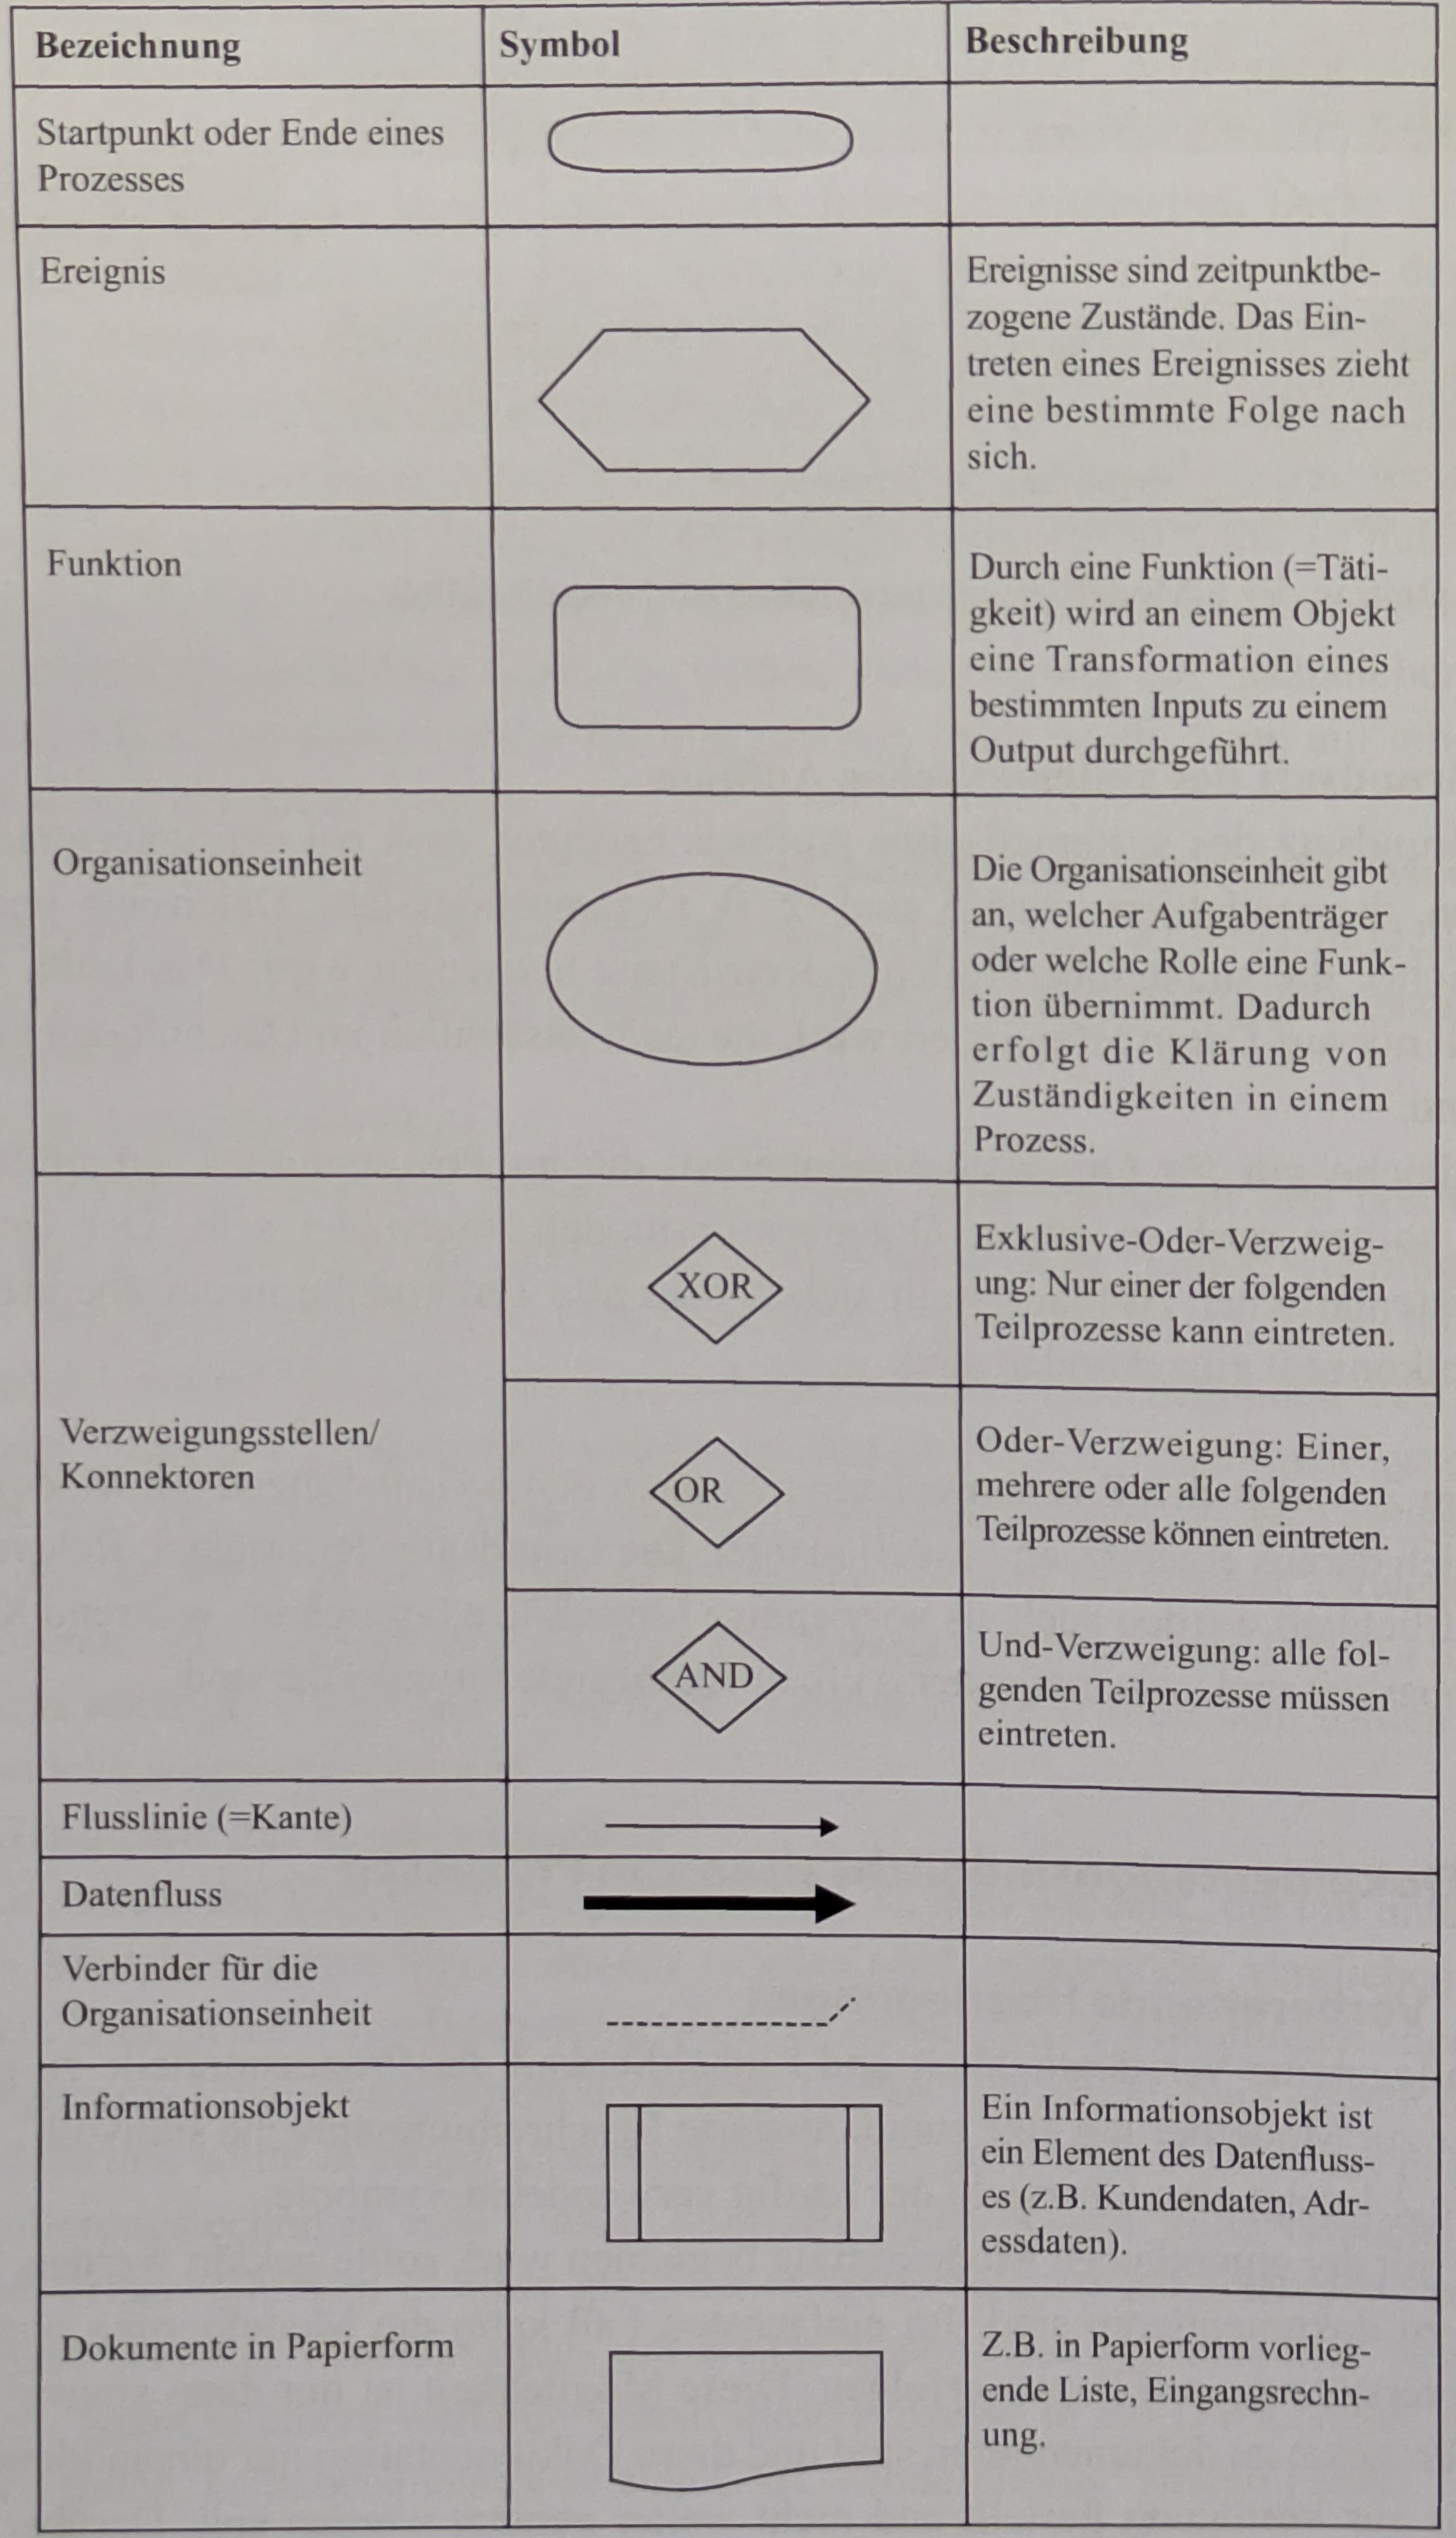
\includegraphics[width=0.8\textwidth]{BILDER-PTB4/symbole_prozessen1.jpg}
\end{center}

\newpage
\vspace*{\fill}
\begin{center}
    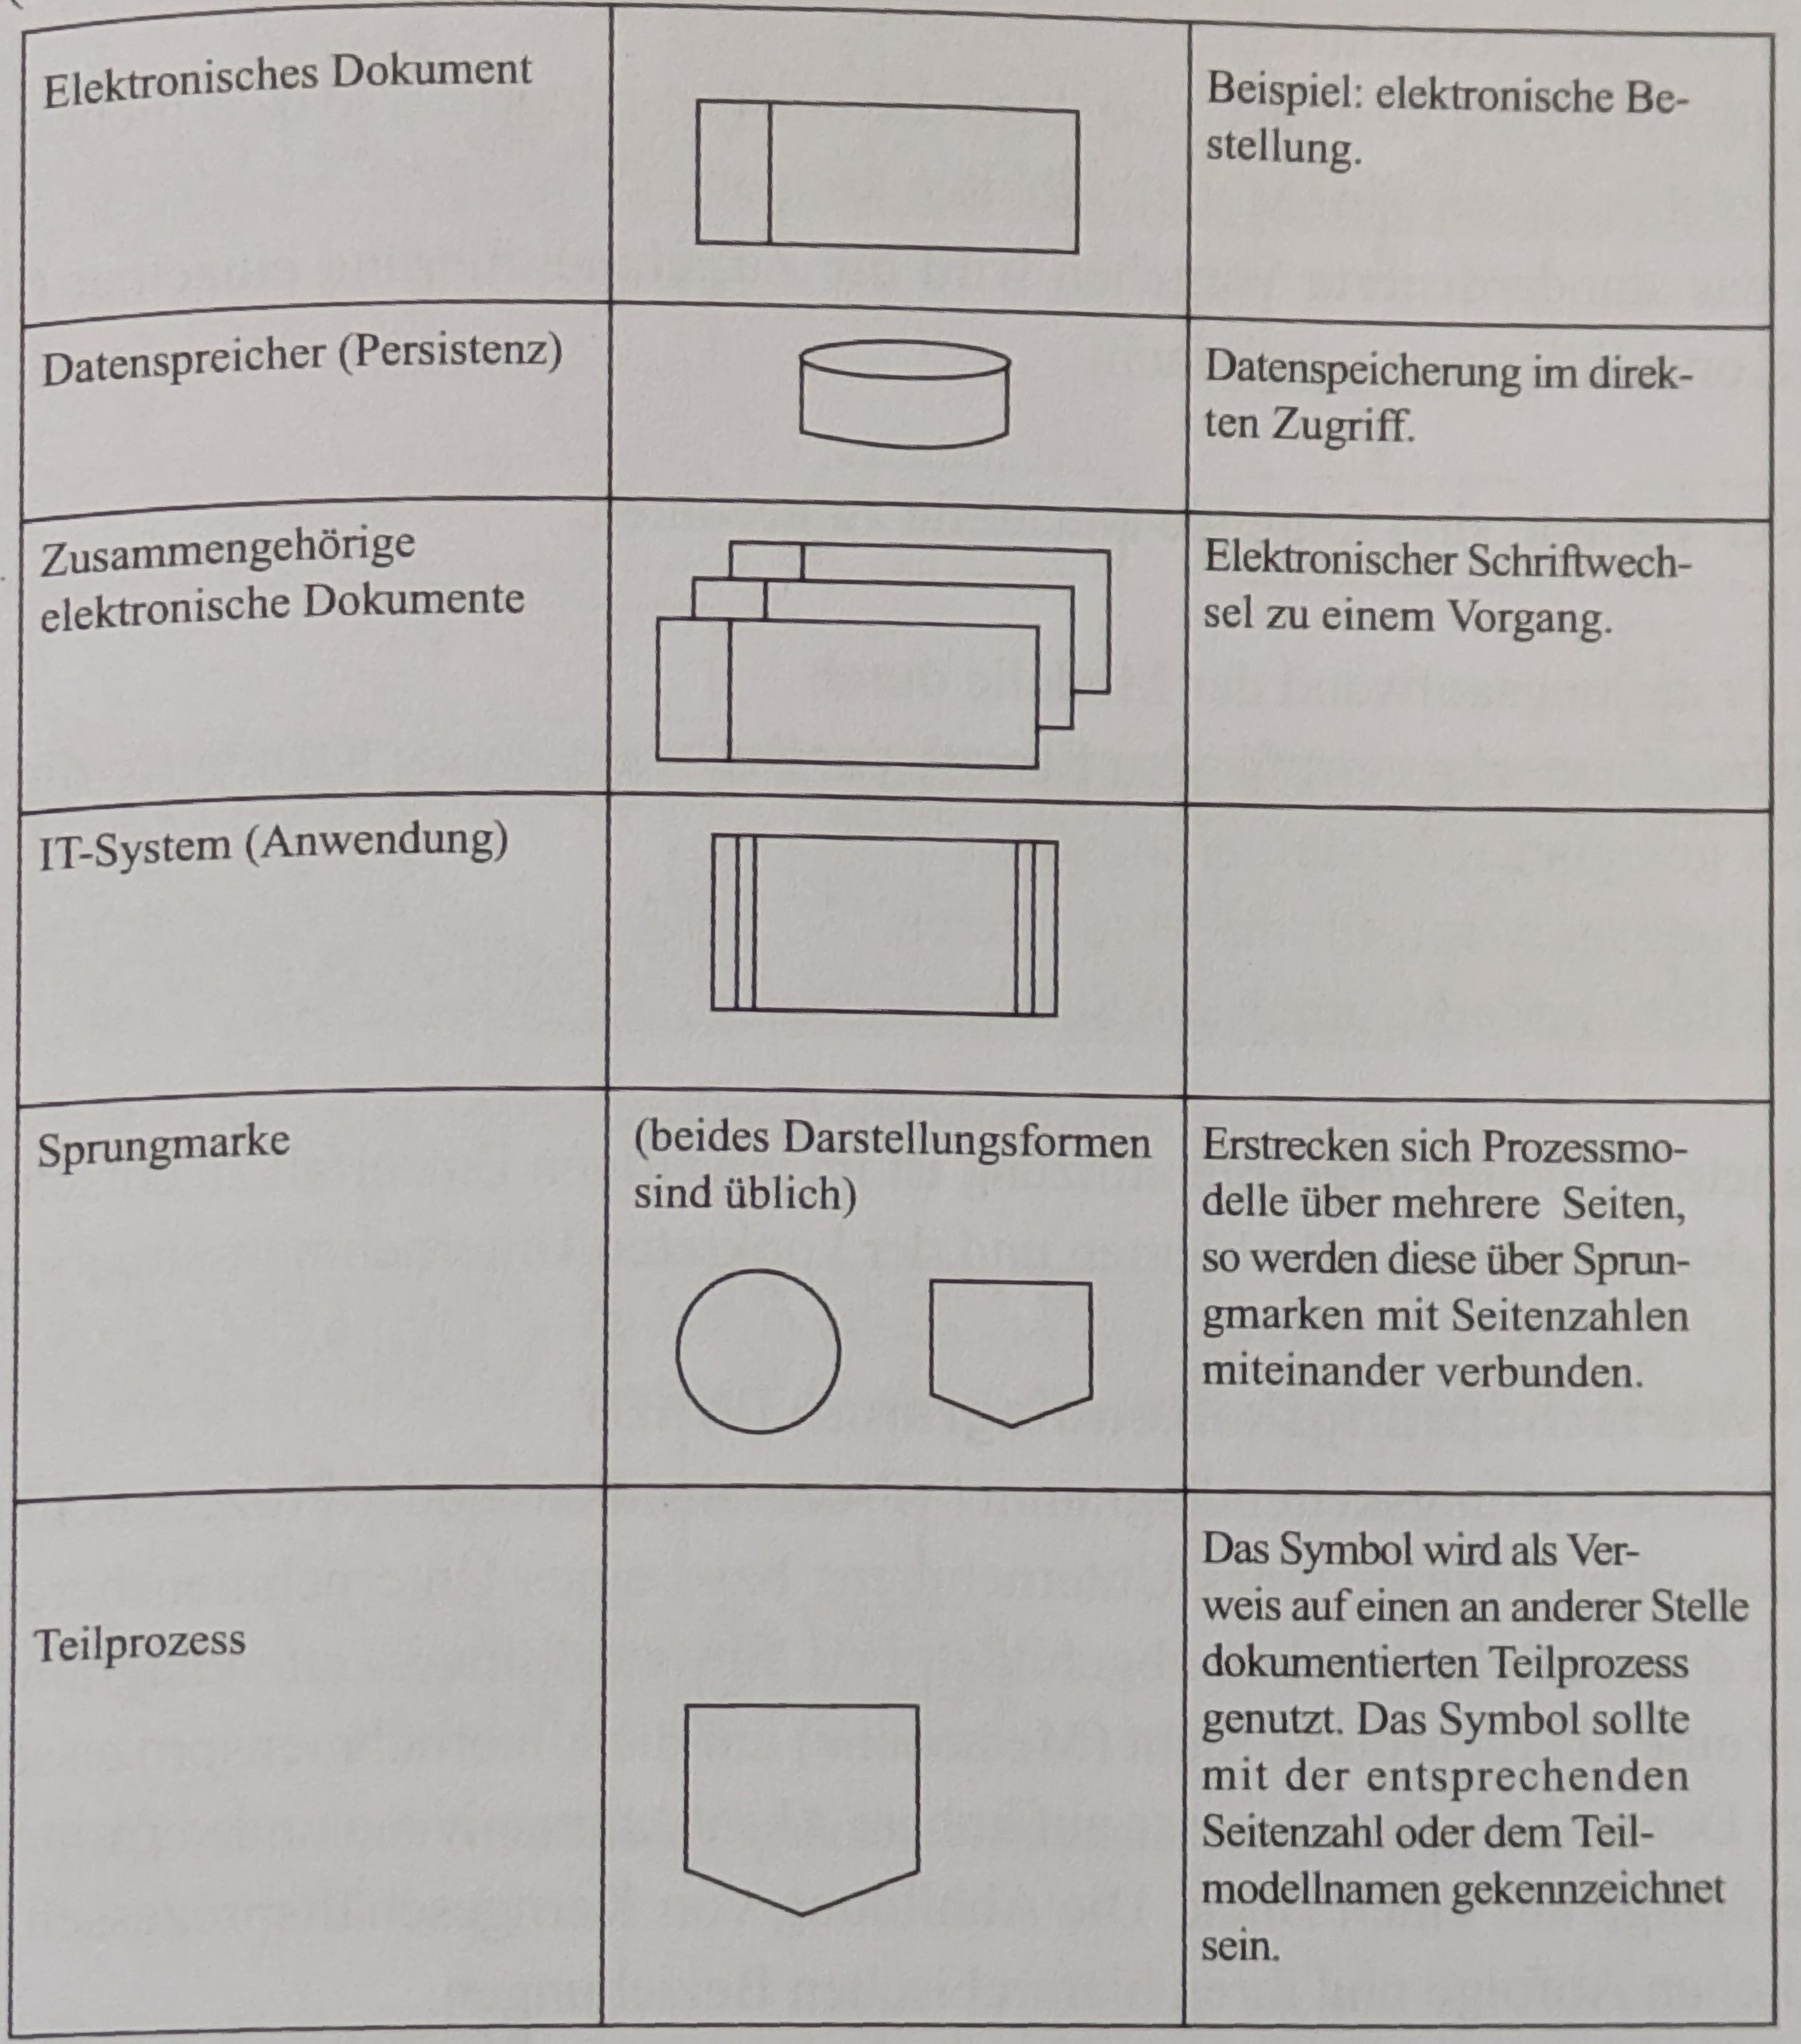
\includegraphics[width=0.85\textwidth]{BILDER-PTB4/symbole_prozessen2.jpg}
\end{center}
\vspace*{\fill}

% Anhang 2
\newpage
\phantomsection
\addcontentsline{toc}{subsection}{Anhang 2: Beteiligungsprozess bei den BWB}
\label{sec:Anhang2}
\begin{center}
    {\Large\bfseries Anhang 2: Beteiligungsprozess bei den BWB}\\[0.2cm]
    {\normalsize Interne Quelle: Beteiligungsprozess-Darstellung zur Einführung neuer Anwendung}\\[0.4cm]
    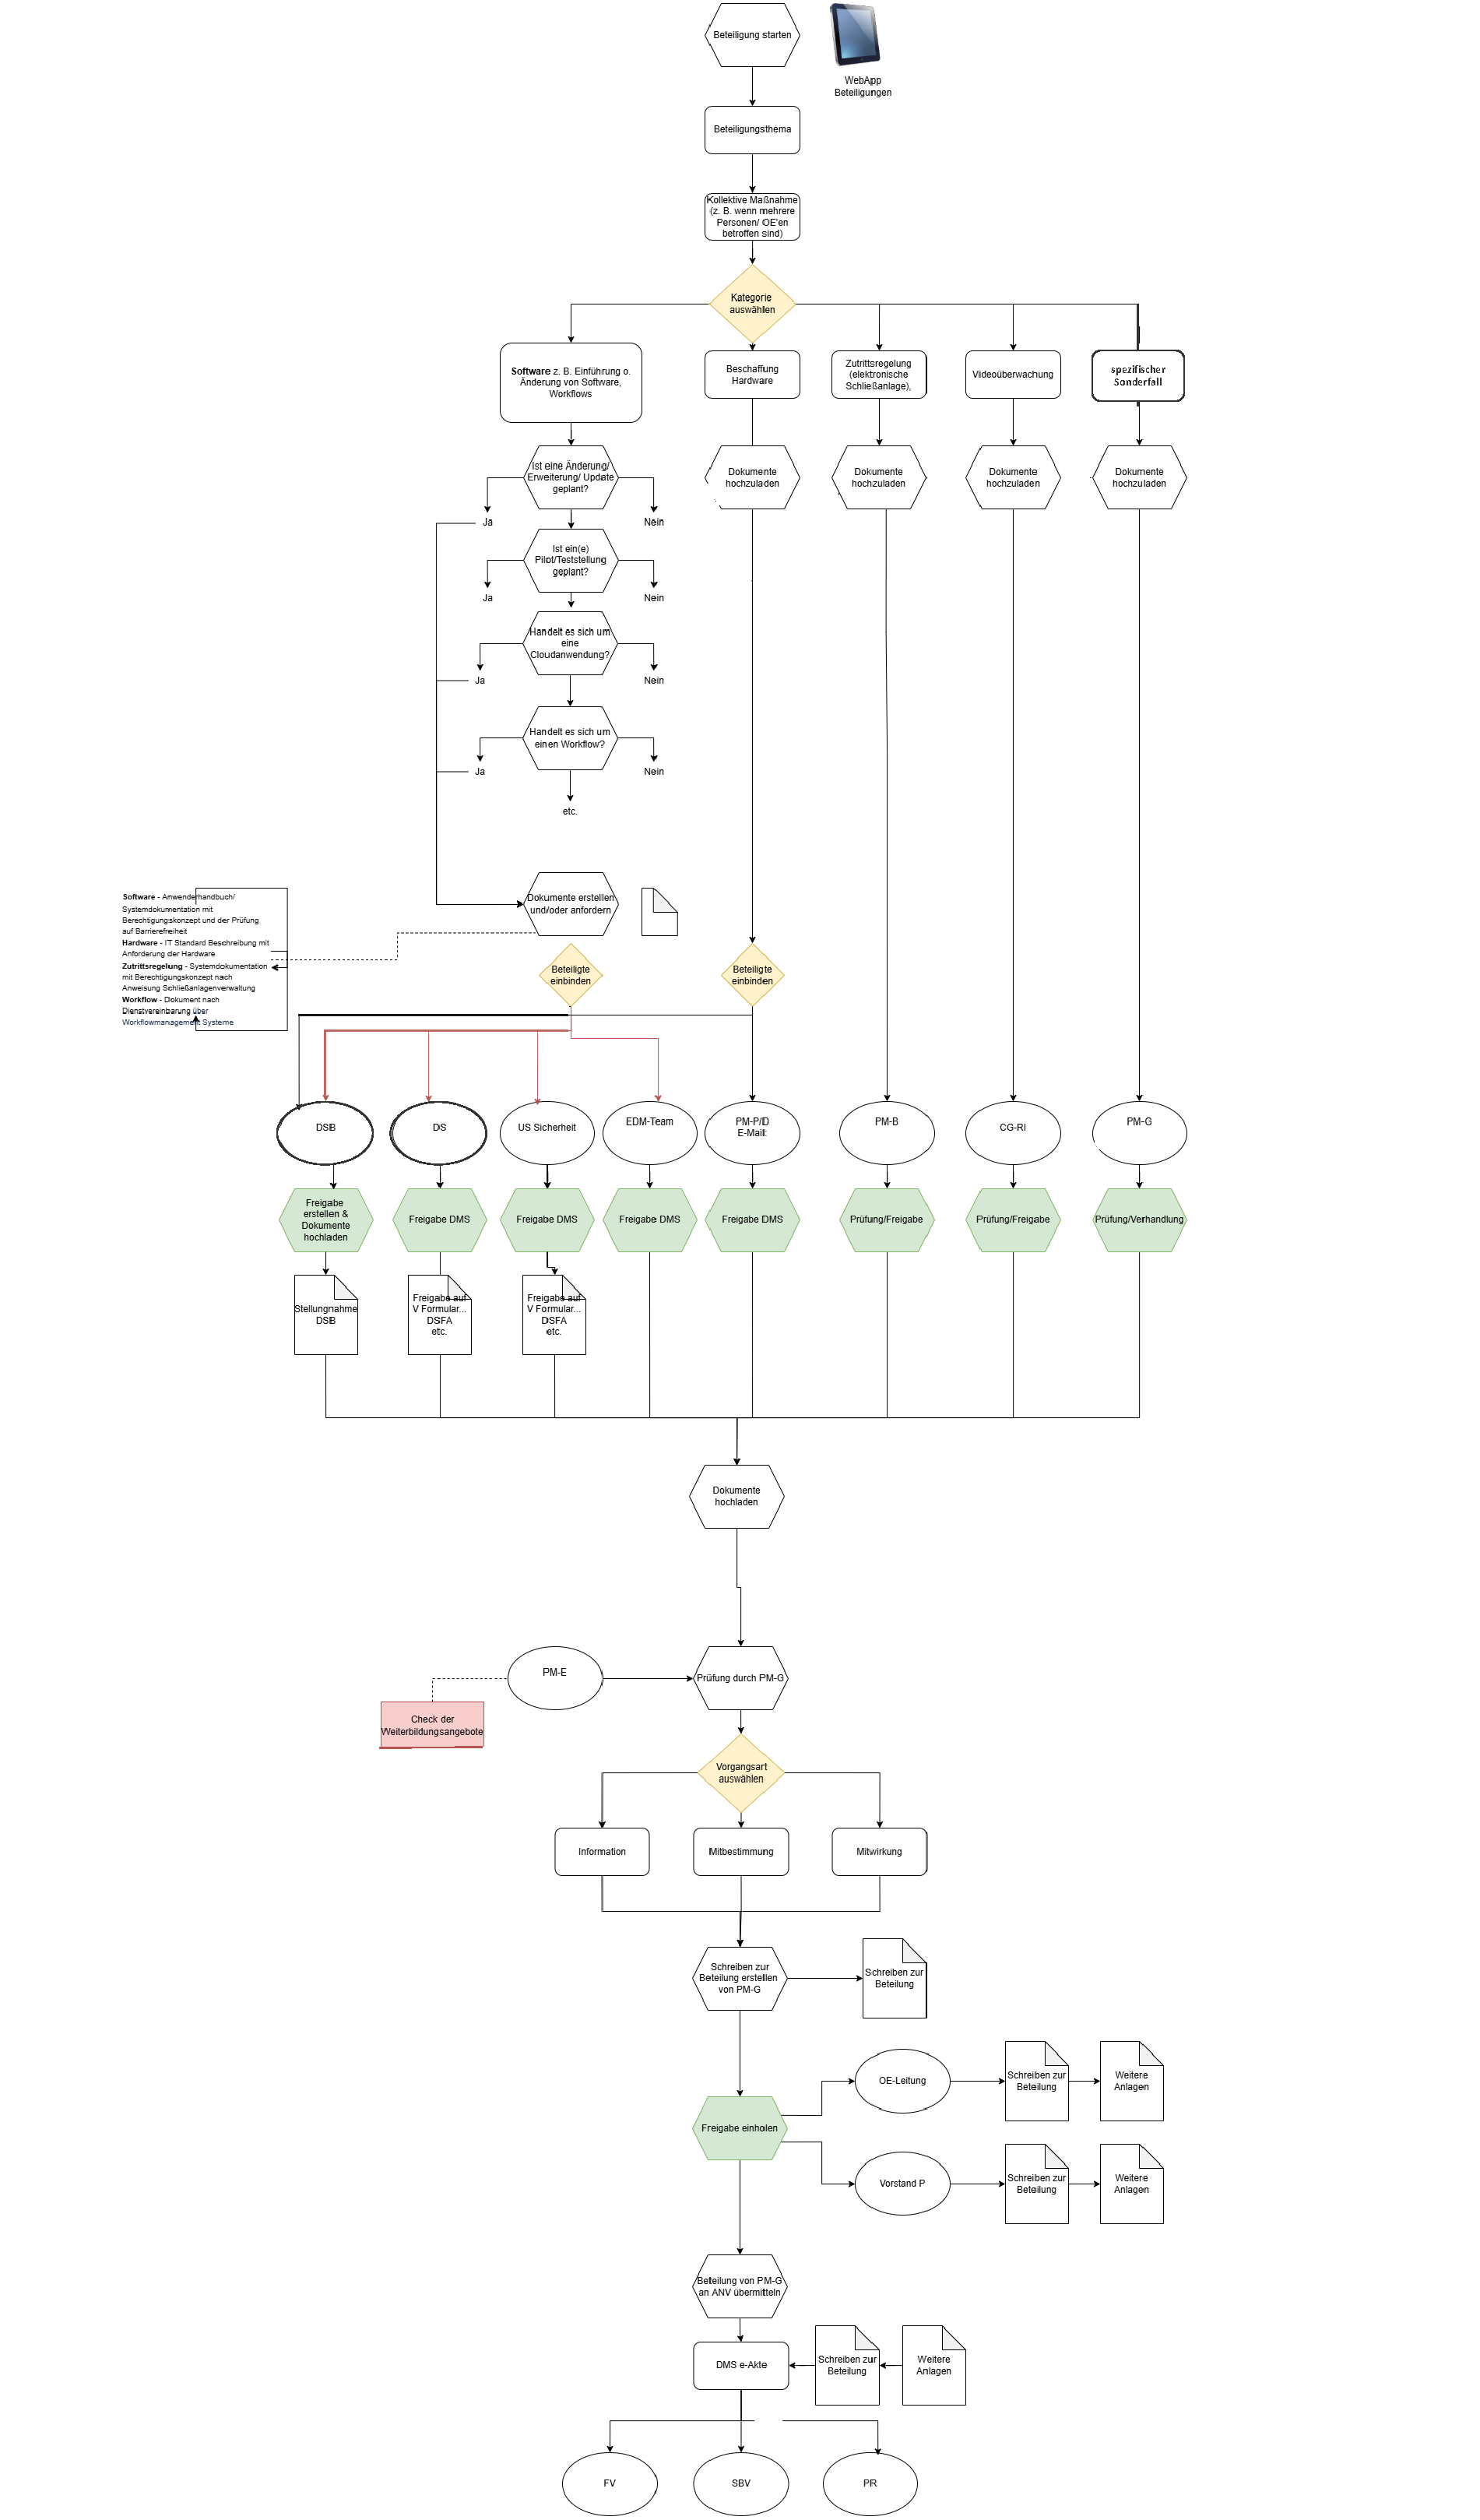
\includegraphics[width=0.82\textwidth]{BILDER-PTB4/beteiligungsprozess_neu.pdf}
\end{center}

% Anhang 3
\newpage
\phantomsection
\addcontentsline{toc}{subsection}{Anhang 3: SWOT-Modell in Matrixdarstellung}
\label{sec:Anhang3}
\vspace*{\fill}
\begin{center}
    \begin{adjustbox}{rotate=90, center, valign=b}
        \begin{minipage}{0.95\textheight}
            \centering
            {\Large\bfseries Anhang 3: SWOT-Modell in Matrixdarstellung}\\[1em]
             {\normalsize Quelle: Eigene Darstellung in Anlehnung an das SWOT-Modell}\\[0.4cm]
            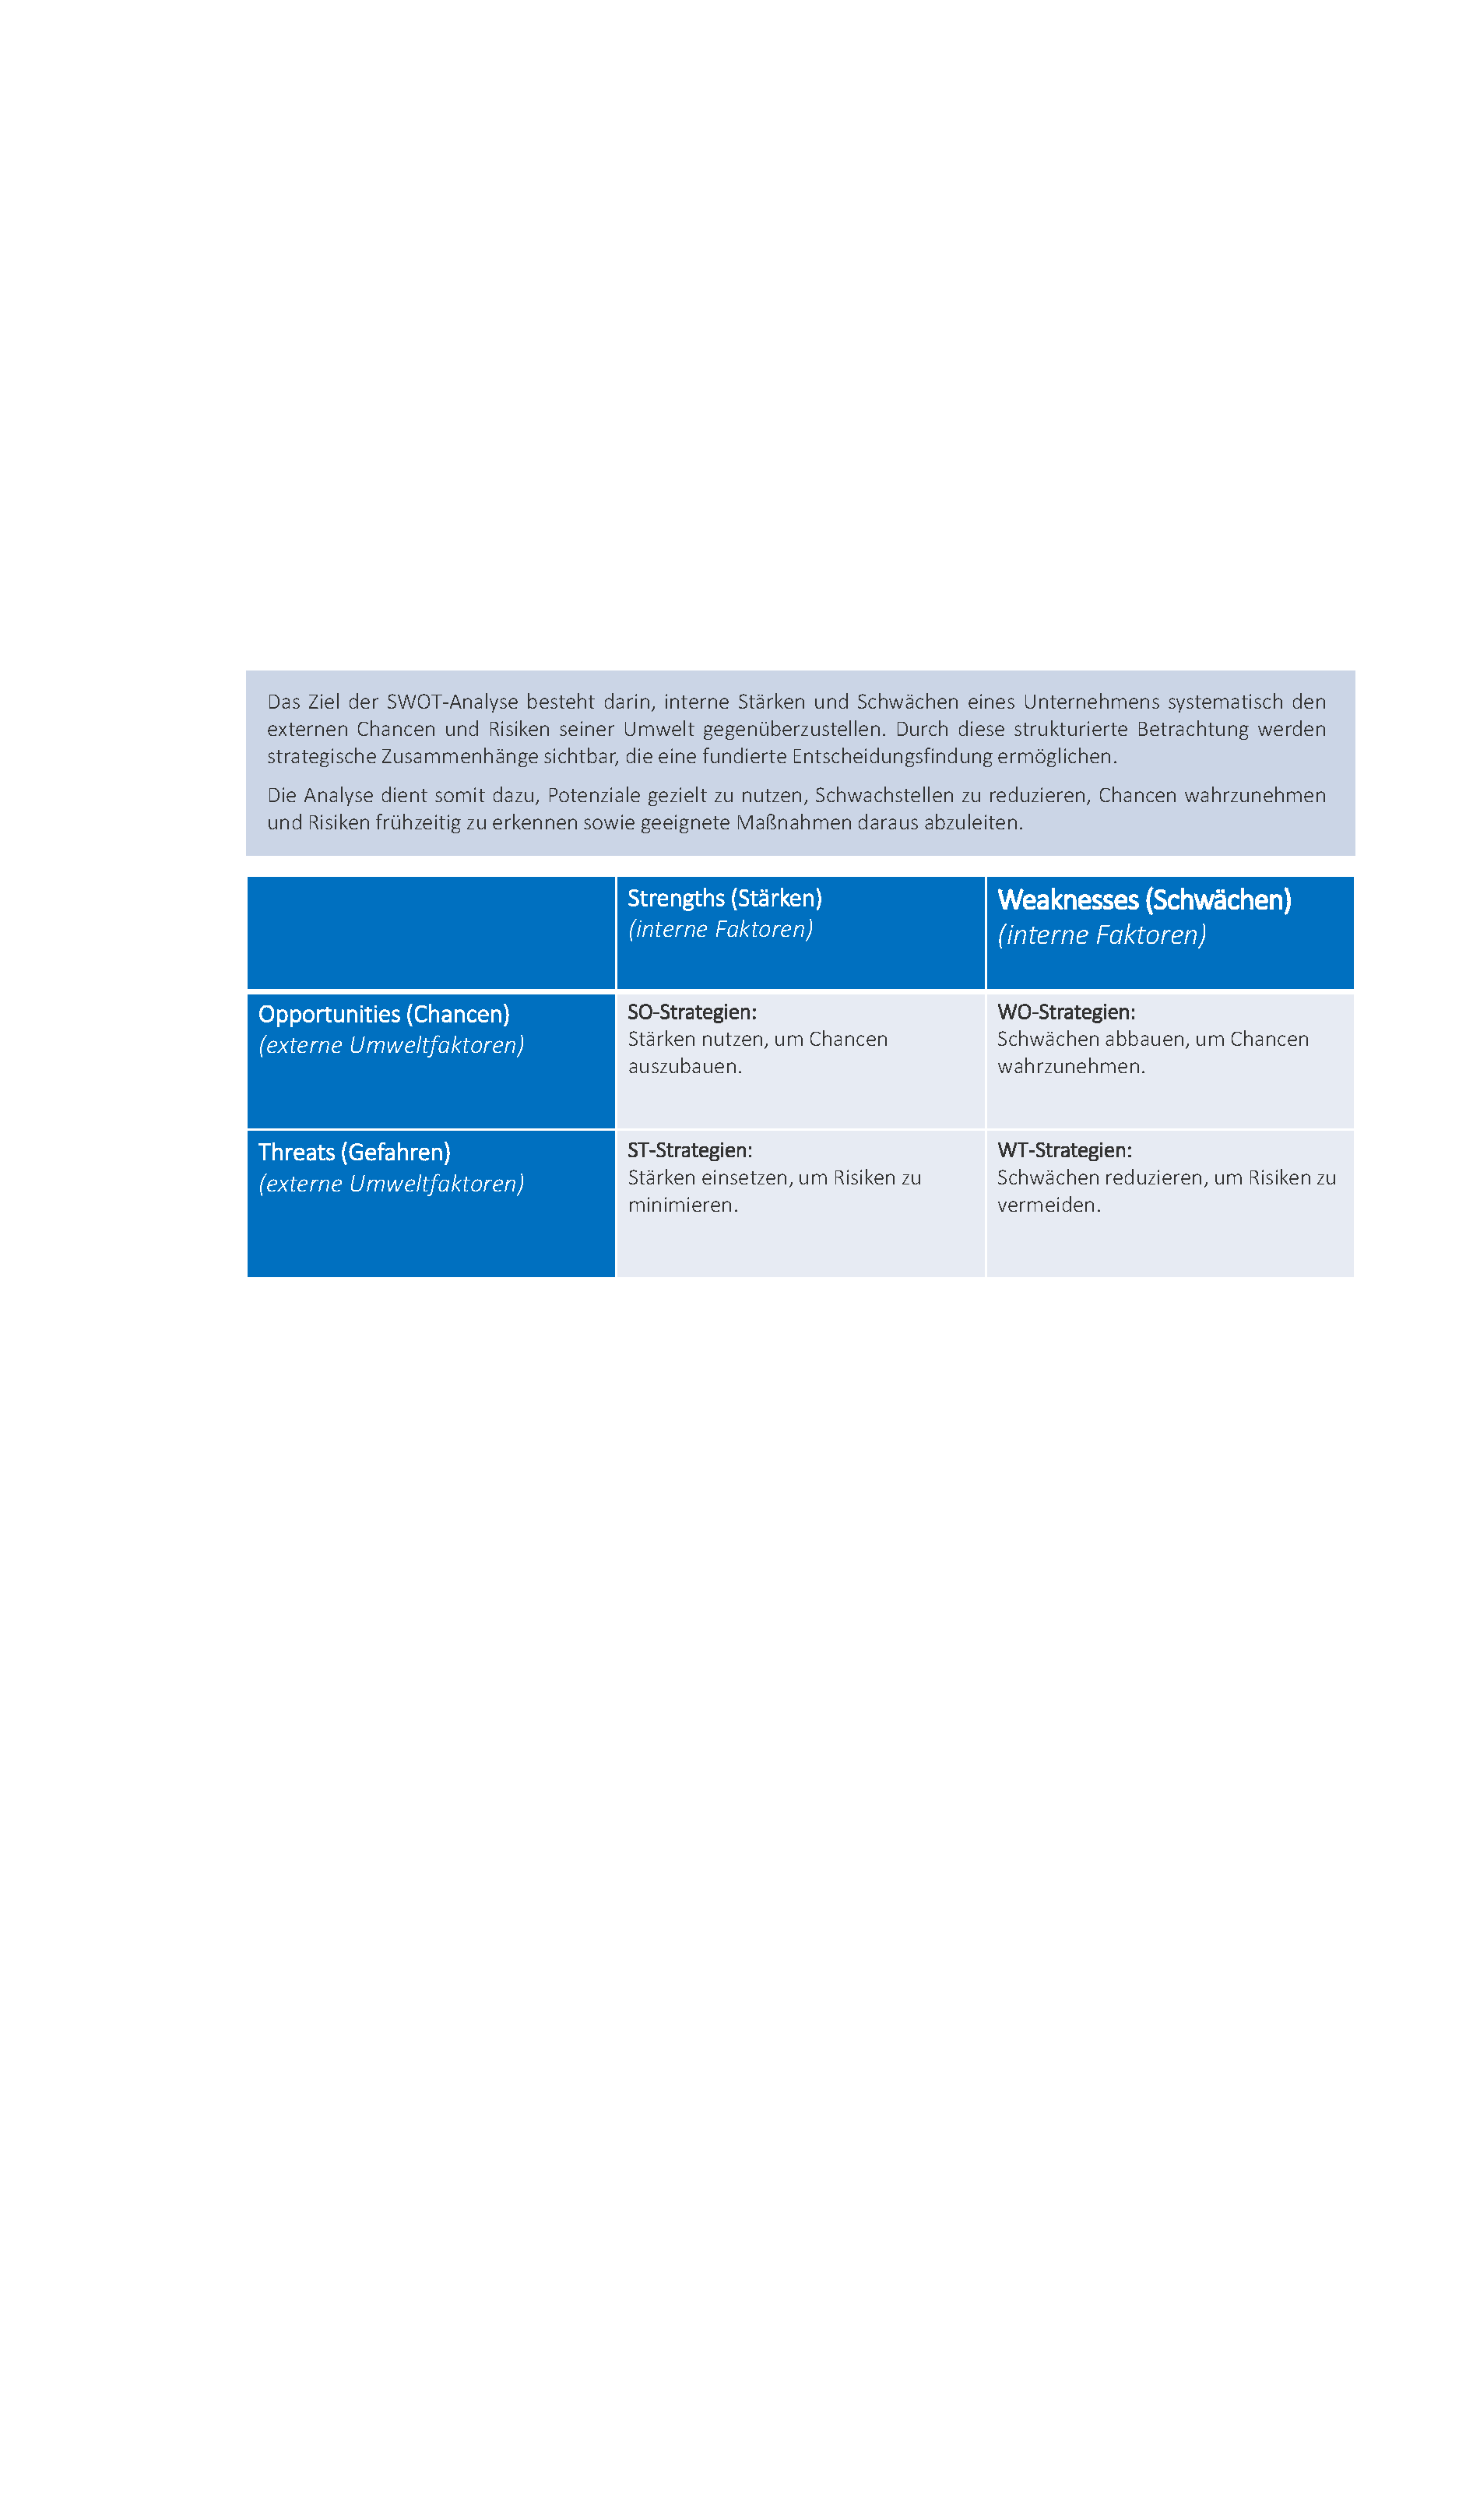
\includegraphics[width=\textheight]{BILDER-PTB4/swot_matrix.pdf}
        \end{minipage}
    \end{adjustbox}
\end{center} 

% Anhang 4
\newpage
\phantomsection
\addcontentsline{toc}{subsection}{Anhang 4: Schulungs- und Kommunikationsprozess bei den BWB}
\label{sec:Anhang4}
\begin{center}
    {\large\bfseries Anhang 4: Schulungs- und Kommunikationsprozess bei den BWB}\\[0.2cm]
    {\normalsize Quelle: Eigene Zusammenfassung des Einführungsprozesses neuer Microsoft-365-Apps mit Schulungs- und Kommunikationsprozess} \\[0.2cm]
    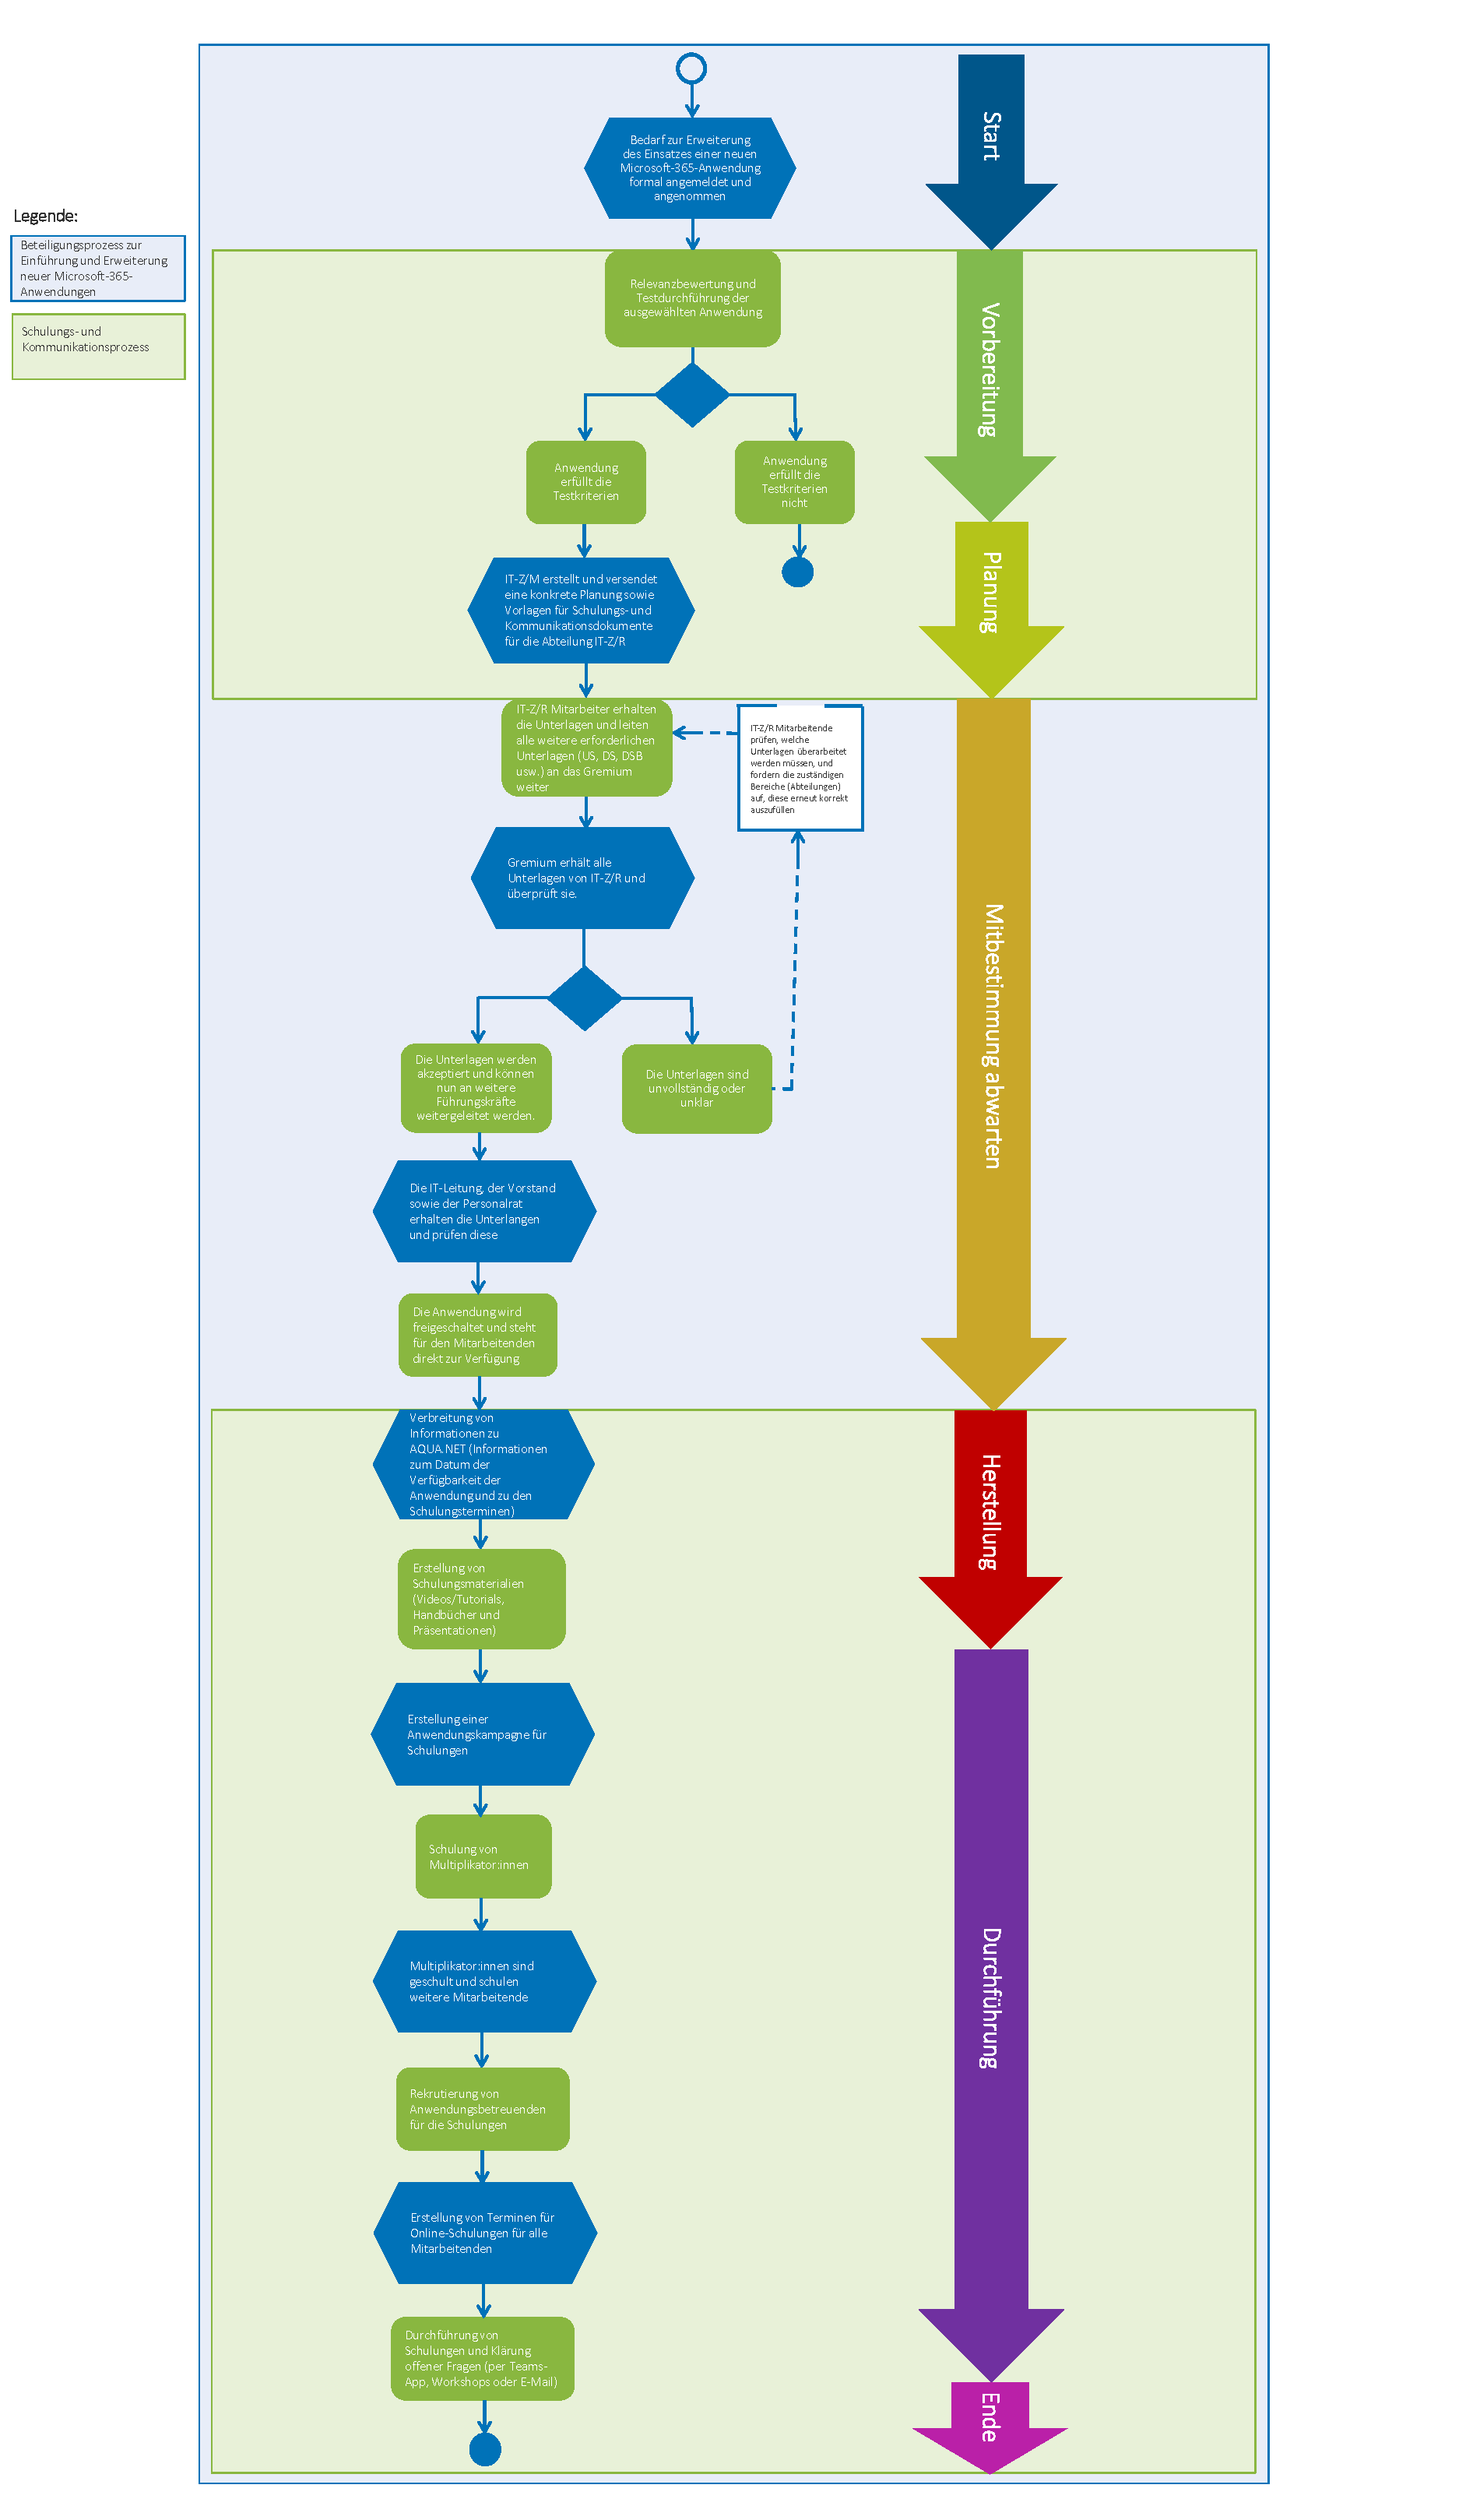
\includegraphics[width=0.81\textwidth]{BILDER-PTB4/schulungs-kommunikationsprozessen_neu.pdf}
\end{center}

% Anhang 5
\newpage
\phantomsection
\addcontentsline{toc}{subsection}{Anhang 5: Interviewprotokoll (Diana Jimenez)}
\label{sec:Anhang5}

{\Large\bfseries Anhang 5: Interviewprotokoll}\\[1em]
\textbf{Interviewer:} Nicole Camille Baião \\
\textbf{Befragte:} Diana Ireri Jimenez Ireta (Leiterin und Beraterin von Microsoft-365-Apps, IT-Z/M) \\
\textbf{Datum:} 03. Februar 2026 \\
\textbf{Ort:} Berliner Wasserbetriebe, Neue Jüdenstraße 2, 10179 Berlin \\

\textbf{Frage 1: Welche Rolle hatten Sie bei der Einführung von Microsoft Planner und To Do?}

Diana Jimenez: Im Jahr 2022 habe ich in unserer IT-Abteilung (IT-Z/M) die Verantwortung dafür übernommen, die Microsoft-365-Anwendungen im Unternehmen einzuführen und Schulungen sowie Betreuung dafür zu koordinieren. Obwohl die BWB das Microsoft-365-Paket bereits seit einiger Zeit besitzt, wurden die einzelnen Anwendungen erst im Rahmen des Beteiligungsprozesses nach und nach freigeschaltet. Zusammengefasst bezeichnet der Beteiligungsprozess den Ablauf zur Einführung oder Erweiterung neuer Anwendungen bei den BWB – von der Abstimmung bis zur Einbindung in Schulungs- und Kommunikationsprozesse. Die Einführung von Planner und To Do stellt daher eine neue Anwendungseinführung bzw. eine Erweiterung der bestehenden Systemlandschaft dar. Zunächst habe ich eng mit einem Kollegen zusammengearbeitet, der als Projektleiter im Modern-Workplace-Projekt tätig war. Schritt für Schritt habe ich dann immer mehr Aufgaben übernommen. Von Anfang an war ich in die Planung eingebunden. Meine Hauptaufgabe war es vor allem, die praktische Umsetzung der Einführung zu übernehmen: zu organisieren, \textit{wie wir die neuen Apps den BWB-Mitarbeiterinnen und -Mitarbeitern bereitstellen und vermitteln}.

Der gesamte Schulungs- und Kommunikationsprozess hängt eng mit dem Beteiligungsprozess zusammen. Sobald ein Bedarf für eine neue Anwendung festgestellt wird, bin ich direkt beteiligt. Ich führe dann mit meinem Team Tests durch und überprüfe, ob das Tool relevant ist und sich eine Einführung lohnt. Wenn das passt, beginne ich, konkrete Schulungsmaterialien zu erstellen, stimme mich mit IT-Z/R ab und versende die Unterlagen zur Genehmigung. Danach muss ich abwarten, bis die Mitbestimmung durchlaufen ist und wir die offizielle Freigabe erhalten. Ohne die Mitbestimmung darf ich nicht mit der Erstellung von Schulungsmaterialien und der Kommunikation mit den Mitarbeitenden beginnen. Die Schulungsmaterialien umfassen vor allem Benutzerhandbücher, Präsentationen und Tutorial-Videos. 

Sobald wir die Freigabe haben, geht es weiter mit dem Schulungs- und Kommunikationsprozess: Wir schulen die Multiplikatoren, also ausgewählte Mitarbeiterinnen und Mitarbeiter, die dann weitere Kolleginnen und Kollegen in ihren Abteilungen schulen. Wenn alle Schulungsmaterialien fertig sind, organisiere ich Werbung für die neuen Online-Schulungen und halte das Ganze in Bewegung. Es ist also kein linearer Prozess, eher ein permanentes Mitdenken und Nachjustieren. Eine externe Beraterin – ein Dienstleister, den die BWB beauftragt hat – hat uns geholfen, den Schulungs- und Kommunikationsprozess mit dem Beteiligungsprozess zu verbinden. Sie hat uns anfangs beraten, und ich habe die Zusammenarbeit koordiniert. Gemeinsam mit dieser Expertin haben wir überlegt, wie wir Schulungsunterlagen und Erklärvideos am besten erstellen. Auf dieser Grundlage habe ich dann die Schulungsmaterialien ausgearbeitet und die Einführung der Tools intern begleitet.

\textbf{Frage 2: Welche Schulungsmaßnahmen wurden zur Einführung angeboten?}

Diana Jimenez: Wir haben mehrere Schulungsformate parallel eingesetzt. Zum einen gab es Live-Schulungen für Mitarbeitende – teils in Form von Workshops oder Online-Sessions –, in denen wir die Funktionen von Planner und To Do vorgestellt haben. Anfangs haben wir mit Multiplikatoren gearbeitet, also einigen ausgewählten Mitarbeitenden, die wir intensiver geschult haben und die dann in ihren Teams als Ansprechpartner dienen konnten. Zum anderen haben wir den Kolleginnen und Kollegen viele Selbstlern-Materialien an die Hand gegeben. Wie erwähnt, haben wir schriftliche Anleitungen (Handbücher) sowie Präsentationsfolien erstellt, damit jeder die Schritte nachvollziehen kann. Außerdem standen kurze Erklärvideos zur Verfügung, die wir intern bereitgestellt haben. Diese Mischung aus direkten Schulungen und unterstützenden Unterlagen sollte sicherstellen, dass unterschiedliche Lernbedürfnisse abgedeckt werden. Insgesamt haben wir versucht, die Einführung möglichst durchdacht zu begleiten, indem wir sowohl persönliche Erklärungen als auch Unterlagen zum Nachlesen und -schauen angeboten haben.

\textbf{Frage 3: Wie wurden die Mitarbeitenden über Planner und To Do informiert?}

Diana Jimenez: Die interne Kommunikation über die neuen Tools lief hauptsächlich über unser Intranetportal AQUA.net. Dort haben wir mehrfach Artikel veröffentlicht, um die Belegschaft über Planner und To Do zu informieren – z.B. Ankündigungen zur Einführung und Tipps zur Nutzung. AQUA.net ist der zentrale digitale Infokanal bei uns, auf dem alle Neuigkeiten geteilt werden. Im Laufe des Einführungsprozesses haben wir also zu mehreren Zeitpunkten Beiträge eingestellt, um die Mitarbeitenden auf dem Laufenden zu halten. Zusätzlich haben wir natürlich in Meetings und via E-Mail auf Schulungsangebote hingewiesen, aber der Hauptkanal war das Intranet. Wichtig war uns, immer wie der an die neuen Möglichkeiten zu erinnern und Hilfestellungen anzubieten, damit Planner und To Do wahrgenommen werden.

\textbf{Frage 4: Wie bekannt sind die neuen Tools unter den Mitarbeitenden?}

Diana Jimenez: Trotz unserer Informationskampagne muss man sagen, dass nicht alle Mitarbeitenden die neuen Anwendungen kennen. Ich schätze, dass etwa 60–70\,\% der Belegschaft mitbekommen haben, dass es Planner und To Do gibt. Viele wissen aber nicht genau, wofür diese Tools eigentlich gedacht sind oder welchen Mehrwert sie bieten. Ein Problem ist sicherlich, dass zwar alle offiziellen Mitteilungen auf AQUA.net stehen, aber nicht jeder Mitarbeitende liest regelmäßig das Intranet. Einige Kollegen – speziell draußen im technischen Bereich – fühlen sich von der ganzen digitalen Informationsflut eher überfordert und meiden solche Plattformen teilweise. Für diese Gruppen gingen die Informationen möglicherweise unter. Hinzu kommt, dass Planner und To Do freiwillige Tools sind – niemand wird von oben dazu verpflichtet, sie zu nutzen. Entsprechend haben manche von vornherein nicht genauer hingeschaut. Insgesamt würde ich sagen, rund zwei Drittel haben zumindest von den Tools gehört. Aktiv nutzen tun sie aber deutlich weniger Mitarbeiter. Mein Gefühl ist, dass momentan vielleicht maximal zehn Prozent der Beschäftigten Planner oder To Do tatsächlich regelmäßig einsetzen. Die Einführung liegt ja auch erst wenige Monate zurück, da ist viel noch in der Ausprobierphase. Nach meiner Erfahrung dauert es in unserem Unternehmen um die fünf Jahre, bis sich ein neues Tool wirklich breit etabliert hat und selbstverständlich genutzt wird.

\textbf{Frage 5: Warum erkennen manche Mitarbeitende den Mehrwert von Planner und To Do nicht?}

Diana Jimenez: Viele Kollegen stehen neuen Tools anfangs skeptisch gegenüber. Wenn etwas Neues kommt, reagieren manche beinahe ängstlich, als wäre es eine völlig fremde Welt. Ich erlebe oft, dass Veränderungen Überforderung auslösen – die Leute fühlen sich von neuen Anwendungen eher erschlagen. Aus Gesprächen mit Kolleginnen und Kollegen habe ich den Eindruck, dass sich viele mehr Unterstützung an der Hand wünschen würden, also eine ganz enge Anleitung nach dem Motto: „Klick zuerst hier, dann dort…“ Diese Führung haben wir auch versucht zu bieten, etwa durch Schritt-für-Schritt-Demos in den Schulungen. Dennoch beobachtet man eine große Bandbreite: Während ein Teil der Mitarbeitenden sehr technikaffin ist und neue Tools wie Planner sofort intuitiv ausprobiert, tun sich andere viel schwerer damit. Es gibt quasi zwei Lager – oft auch entlang der Generationen.

Jüngere Kollegen haben meist Spaß daran, neue digitale Hilfsmittel auszuprobieren, und bringen sich vieles selbst bei. Ältere Mitarbeitende dagegen empfinden solche Tools häufiger als kompliziert und lästig. Ihre Hemmschwelle ist höher, und sie bleiben lieber bei den gewohnten Arbeitsweisen. In der Tat hat es bei uns z. B. Jahre gedauert, bis Confluence (das interne Wiki) von allen akzeptiert und genutzt wurde – anfangs hieß es auch, das sei unübersichtlich und so weiter. Erst nach fünf Jahren war das Tool wirklich integriert im Arbeitsalltag. Jetzt kommen wir mit noch neueren Anwendungen wie Planner, die ähnliches können, und da fragen erfahrene Kollegen natürlich: „Wozu das Ganze? Warum sollen wir schon wieder wechseln?“ Dieses Gefühl, bereits Bewährtes zu haben, lässt manche den Nutzen eines weiteren Tools infrage stellen. Wie gesagt, einige informieren sich auch schlicht nicht, weil sie gar kein Interesse daran haben. Und diejenigen, die Bescheid wissen, nutzen Planner und To Do teilweise trotzdem nicht, weil sie es nicht möchten – es ist ja, wie erwähnt, kein Zwang. Diese Vorbehalte und die Zurückhaltung gehören zu den größten Hürden bei der Verbreitung der neuen Tools.

\textbf{Frage 6: Was waren die größten Herausforderungen bei den Schulungen?}

Diana Jimenez: In den Schulungen selbst war die Teilnehmende auf ganz unterschiedlichen Kenntnisstufen eine echte Herausforderung. Häufig saßen in einer Session Kollegen mit sehr unterschiedlichen Vorkenntnissen zusammen. Da den richtigen Tempo-Mix zu finden, war schwierig: Entweder war ich für die einen zu langsam, oder für die anderen zu schnell. Zum Beispiel hatten einige das Prinzip sofort intuitiv verstanden, während andere bei jeder neuen Funktion erst einmal ins Stocken gerieten. Aus dieser Erfahrung habe ich gelernt und meine Herangehensweise angepasst: Künftig würde ich die Trainingsgruppen nach Wissensstand trennen und vorab abfragen, wer schon Vorerfahrung mitbringt. So kann man Einsteiger und Fortgeschrittene getrennt schulen. Außerdem ist es besser, weniger Inhalte pro Termin zu vermitteln und dafür die Anzahl der Schulungstermine zu erhöhen. Wir haben am Anfang vielleicht zu viel auf einmal zeigen wollen – alle Funktionen in einer Sitzung – und damit einige überfordert. Besser ist es, kleinere Lerneinheiten zu machen. So bleibt jeder dran, ohne dass die einen sich langweilen und die anderen überfordert sind. Diese Aufteilung nach Niveau und Häppchenbildung des Stoffs hat sich für mich als wichtige Lektion aus den ersten Schulungen ergeben.

\textbf{Frage 7: Wie können die Schulungs- und Kommunikationsprozesse verbessert werden?}

Diana Jimenez: Aus heutiger Sicht würde ich vorschlagen, unsere Schulungs- und Kommunikationsstrategie noch gezielter auf die verschiedenen Zielgruppen zuzuschneiden. Zum einen könnten wir bei den Schulungen stärker nach Altersgruppen oder Vorkenntnissen differenzieren. Beispielsweise bräuchten ältere Kollegen oder generell diejenigen mit wenig IT-Erfahrung vielleicht noch ausführlichere Erläuterungen – für sie wären zusätzliche, detaillierte Tutorials oder Videos hilfreich. Jüngeren und versierteren Nutzergruppen reichen oft schon kurze Übersichten oder Workshops, um den Einstieg zu finden. Hier könnten wir also vom Umfang her variieren, damit niemand unterfordert oder überfordert wird. Zum anderen sollten wir bei der internen Kommunikation neue Wege gehen. 

Wie besprochen, ist AQUA.net als einziges Medium nicht genug, weil es gewisse Mitarbeiterkreise nicht erreicht. Man könnte überlegen, weitere Kanäle einzusetzen, um über Neuerungen wie Planner und To Do zu informieren. Zum Beispiel wurde intern die Idee diskutiert, eine Art unternehmensweiten Chat oder Social Feed einzurichten, wo alle Beschäftigten Neuigkeiten mitbekommen. So etwas wie ein zentraler Teams-Kanal für die ganzen Wasserbetriebe existiert zwar, aber er wird nicht von allen genutzt – vielleicht braucht es ein noch niedrigschwelligeres Kommunikationstool, das wirklich jeden erreicht. Kurz gesagt: Wir sollten parallel zum Intranet andere Kommunikationswege ausprobieren, um auch die Mitarbeitenden abzuholen, die bisher kaum Informationen mitbekommen. Wenn wir Schulungsangebote zielgruppengerechter gestalten und die Informationsverbreitung breiter aufstellen, könnten künftige Einführungsprozesse vermutlich deutlich effizienter und erfolgreicher verlaufen.

% Anhang 6
\newpage
\phantomsection
\addcontentsline{toc}{subsection}{Anhang 6: Interviewprotokoll (Nicolas Zoll)}
\label{sec:Anhang6}

{\Large\bfseries Anhang 6: Interviewprotokoll}\\[1em]
\textbf{Interviewer:} Nicole Camille Baião \\
\textbf{Befragter:} Nicolas Zoll (Risikomanager, IT-Z/R) \\
\textbf{Datum:} 05. Februar 2026 \\
\textbf{Ort:} Berliner Wasserbetriebe, Neue Jüdenstraße 2, 10179 Berlin \\

\textbf{Frage 1: Welche Rolle haben Sie im Beteiligungsprozess zur Einführung neuer Softwareprodukte?}

Nicolas Zoll: Meine Aufgabe ist es, den Beteiligungsprozess bei neuen Software-Einführungen zu koordinieren. Ich bin Risikomanager (und auch für Qualitätsmanagement zuständig) und arbeite im Abteilung IT-Z/R (IT-Zentrale Aufgaben – Risk Complance and Security). Unsere Bereichsleitung hat mich und eine Kollegin (Leiterin von IT-Z/R) benannt, um alle Beteiligungsvorgänge zu betreuen. Wir selbst erstellen die erforderlichen Dokumente nicht – das machen die jeweiligen Projekt- oder Fachverantwortlichen des neuen Tools. Stattdessen stellen wir sicher, dass alle Unterlagen vollständig vorliegen, und beraten die Kollegen, was genau eingereicht werden muss. Kurz gesagt: Wir begleiten und steuern den Prozess beratend im Hintergrund, damit am Ende sämtliche nötigen Freigaben und Dokumente für das Beteiligungsverfahren vorhanden sind.

\textbf{Frage 2: Wie läuft der Prozess ab, wenn eine neue Software eingeführt werden soll, und wer ist wann beteiligt?}

Nicolas Zoll: Zunächst muss der Bedarf für das neue Softwareprodukt formal angemeldet werden. Die zuständige Projektleitung (bzw. Fachabteilung) bereitet einen Einführungsantrag vor – in Form eines \textit{„Whitepapers zur Beteiligung“}. In dieser standardisierten Vorlage werden die Grunddaten des Vorhabens festgehalten (Ansprechpartner, betroffene Bereiche, geplantes Einführungsdatum etc.). Parallel dazu erstellt das Projekt eine kurze Beschreibung der Software und ihrer Funktionen sowie ein Berechtigungskonzept. Bereits in dieser frühen Phase werden wichtige Stellen vorab eingebunden: So findet eine Abstimmung mit dem IT-internen Datenschutz-Team, dem sogenannten EDM-Team als technische Experten der Arbeitnehmervertretung) statt, um das Vorhaben technisch mit der Arbeitnehmerseite vorzuklären. Ebenso muss der Datenschutzbeauftragte (DSB) frühzeitig eingebunden werden und eine schriftliche Stellungnahme abgeben, dass aus Datenschutz-Sicht nichts gegen die Einführung spricht. Handelt es sich um eine Cloud-Anwendung, wird zusätzlich die Datenschutz-Fachabteilung (DS) involviert. Außerdem schaltet die IT die Unternehmenssicherheit (Abteilung US) ein: Gemeinsam wird eine Schutzbedarfsfeststellung durchgeführt, um das Sicherheitsniveau des neuen Tools einzuschätzen (Quick-Scan mit entsprechenden Fragen zur Anwendung). Bereits hier werden also Datenschutz und IT-Security eng einbezogen.

Sobald alle Unterlagen ausgearbeitet sind und die nötigen Vorab-Freigaben eingeholt wurden, wird das Gesamtpaket an Dokumenten zunächst in der Personalmanagement-Abteilung - also im Gremium (PM-G) - überprüft, ob die Dokumentenanforderungen erfüllt sind. Als nächstes wird der Vorstand gemeinsam mit dem IT-Leiter jede Software-Einführung vor der offiziellen Einreichung prüfen. Wenn alles korrekt ist, wird der Vorgang in das eigentliche Beteiligungsverfahren an den Personalrat weitergeleitet. Dort wird der Vorgang behandelt – der Personalrat hat die Mitbestimmung und muss dem Einsatz der neuen Software zustimmen - und weitergeleitet (je nach Bereich an den Personalrat der Hauptverwaltung, Wasser oder Abwasser). Durch diese extra Schleife stellen wir sicher, dass die Leitung früh informiert ist und der Personalrat später nicht mit unvollständigen Informationen konfrontiert wird.  Liegt schließlich die Zustimmung des Personalrats vor, darf die Software produktiv ausgerollt werden. Erst nach dieser formalen Freigabe ist die Einführung offiziell abgeschlossen und das Tool kann unternehmensweit genutzt werden.

\textbf{Frage 3: Welche Dokumente und Materialien müssen für das Beteiligungsverfahren vorbereitet werden?}

Nicolas Zoll: Für die Einführung eines neuen Tools ist eine ganze Reihe von Unterlagen erforderlich. Insbesondere müssen wir folgende Dokumente bündeln:
\begin{itemize}
    \setlength\itemsep{0.4\baselineskip}
    \setlength\parskip{0pt}
    \setlength\parsep{0pt}
    \item \normalsize ein Whitepaper zur Beteiligung – die offizielle Vorlage mit den Basisinformationen zum Vorhaben (Art der Software, Bedarf, Ansprechpartner, Zeitplan usw.),
    \item \normalsize eine fachliche Beschreibung der Software (inklusive der vorgesehenen Funktionalitäten und eines Berechtigungskonzepts zur Rechtevergabe),
    \item \normalsize eine Schutzbedarfsfeststellung – also die Bewertung des erforderlichen Sicherheitsniveaus einer Anwendung im Hinblick auf IT-Sicherheit und Datenschutz – in Zusammenarbeit mit der Unternehmenssicherheit; oft in Form eines Quick-Scans mit definierter Checkliste,
    \item \normalsize sämtliche Datenschutz-Dokumente: insbesondere das Verzeichnis von Verarbeitungstätigkeiten (VVT) – die Dokumentation aller Verarbeitungsvorgänge personenbezogener Daten innerhalb der Organisation –, 
    \item \normalsize ein entsprechendes Löschkonzept zur Regelung der datenschutzkonformen Löschung personenbezogener Daten mit definierten Fristen und Verfahren sowie eine initiale Datenschutz-Risikoanalyse; falls diese ergibt, dass ein hohes Risiko für die Rechte und Freiheiten betroffener Personen vorliegt, kommt noch eine ausführliche Datenschutz-Folgenabschätzung als vertiefte Risikoanalyse hinzu,
    \item \normalsize die schriftlichen Freigaben/Stellungnahmen der Datenschutzinstanzen – also eine Einwilligung des Datenschutzbeauftragten (DSB) und ggf. zusätzlich eine Stellungnahme der Datenschutz-Abteilung (DS), falls diese beteiligt werden muss (z. B. bei Cloud-Themen),
    \item \normalsize ein Schulungskonzept und Anwender-Unterlagen für die Beschäftigten – beispielsweise Benutzerhandbücher, Präsentationen oder Lernvideos. Diese Materialien dienen dazu, die Mitarbeiter auf das neue Werkzeug vorzubereiten. Die Arbeitnehmervertretung fragt im Beteiligungsverfahren gezielt nach solchen Schulungsmaßnahmen, um sicherzustellen, dass alle Anwender mit der eingeführten Software umgehen können.
\end{itemize}
Alle diese Unterlagen müssen von den Projektverantwortlichen vorbereitet und im Zuge des Antrags eingereicht werden. Unsere Aufgabe in IT-Z/R ist es, darauf zu achten, dass diese Dokumente vollständig vorliegen und inhaltlich mit den zuständigen Stellen (DSB, DS, US etc.) abgestimmt sind, bevor wir den Antrag weiterleiten.

\textbf{Frage 4: Welche typischen Probleme treten im aktuellen Beteiligungsprozess auf?}

Nicolas Zoll: Aus meiner Sicht ist der Prozess momentan sehr aufwendig und zeitintensiv. Ein Hauptproblem ist der hohe Abstimmungsaufwand: Es sind zu viele Parteien involviert – vom Datenschutzbeauftragten über die Datenschutz-Abteilung und die Unternehmenssicherheit bis hin zu mehreren Gremien der Personalvertretung. Jede dieser Stellen muss nacheinander eingebunden werden, was zu erheblichen Verzögerungen führt. Je mehr Leute mitreden, desto länger dauert am Ende die Einführung. Hinzu kommt ein enormer Dokumentationsaufwand: Für jedes Vorhaben müssen unzählige Formulare, Konzepte und Stellungnahmen erstellt werden. Viele dieser Unterlagen überschneiden sich inhaltlich, was zu Medienbrüchen und Doppelarbeit führt – man pflegt ähnliche Informationen in verschiedenen Dokumenten und Systemen parallel. Das macht den Ablauf in der Praxis sehr mühsam und fehleranfällig.

\textbf{Frage 5: Wie könnte der Beteiligungsprozess verbessert oder beschleunigt werden?}

Nicolas Zoll: Ich sehe durchaus Potenzial, den Prozess schlanker und effizienter zu gestalten. Ein wichtiger Schritt, der bereits angegangen wird, ist die Digitalisierung des Verfahrens: Statt in zig Word-Dokumenten und Excel-Listen alles manuell auszufüllen, sollte ein einheitlicher Workflow im System den Prozess abbilden. Wenn alle Informationen in einer zentralen Plattform erfasst und automatisch an die zuständigen Stellen weitergeleitet werden, reduzieren wir die Medienbrüche und sparen viel Zeit. Zum Glück wird so ein Workflow-System jetzt endlich eingeführt – darauf setze ich große Hoffnungen. Zudem würde ich die Anzahl der Beteiligten Instanzen reduzieren, um Doppelarbeit zu vermeiden. Beispielsweise könnte man die Datenschutz-Prüfung auf eine Instanz konzentrieren. Es würde reichen, wenn der Datenschutzbeauftragte das Vorhaben bewertet und freigibt – die zusätzliche Prüfung durch die separate Datenschutz-Abteilung könnte entfallen, denn zwei parallele Datenschutzbewertungen sind aus meiner Sicht überflüssig (zumal DSB und DS oft das Gleiche prüfen). Allgemein sollten nicht „zu viele Köche“ mitreden, da dies den Brei nur verdirbt – sprich: weniger involvierte Personen würden den Ablauf vereinfachen und beschleunigen.

Ein weiterer Verbesserungsansatz betrifft den Dokumentationsaufwand. Hier sollte geprüft werden, welche Unterlagen wirklich erforderlich sind. Viele Dokumente (etwa das VVT und das Löschkonzept) sind in der jetzigen Form für die Tool-Einführung nicht ideal, weil sie stets für einen einzelnen Geschäftsprozess gedacht sind. Man könnte überlegen, statt für jedes neue Tool komplett neue umfangreiche Dokumente zu schreiben, eher mit vereinfachten Checklisten oder Referenzen auf bestehende Prozess-Dokumentationen zu arbeiten. Zusammengefasst würde ich mir einen schlankeren Prozess mit weniger Bürokratie wünschen. Weniger Beteiligte, klarere Zuständigkeiten und frühzeitige Abstimmung der wichtigen Punkte (Datenschutz, IT-Sicherheit) in einem digital unterstützten Workflow würden viel helfen. So könnten neue Microsoft-365-Tools deutlich schneller und reibungsloser eingeführt werden, ohne dass wichtige Prüfschritte ausgelassen werden – einfach mit weniger Overhead.

% Anhang 7
\newpage
\phantomsection
\addcontentsline{toc}{subsection}{Anhang 7: KI-Verzeichnis}
\label{sec:Anhang7}

{\Large\bfseries Anhang 7: KI-Verzeichnis}\\[0.6cm]

\begin{tabular}{|p{3.2cm}|p{5.2cm}|p{4.2cm}|p{3.2cm}|}
    \hline
    \textbf{KI-basiertes Hilfsmittel} & \textbf{Einsatzform} & \textbf{Betroffene Teile der Arbeit} & \textbf{Bemerkungen} \\
    \hline
    ChatGPT (OpenAI) & Verbesserung der Textformulierung und Grammatik. & Ganze Arbeit. & Nur Sprachkorrektur, keine inhaltliche Änderung. \\
    \hline
    DeepL Translator & Übersetzung von Textpassagen. & Ganze Arbeit. & Übersetzung einzelner Wörter sowie kurzer Sätze. \\
    \hline
\end{tabular}

% === Ehrenwörtliche Erklärung ===
\newpage
\section*{Ehrenwörtliche Erklärung}
\phantomsection
\addcontentsline{toc}{section}{Ehrenwörtliche Erklärung}

„Ich erkläre ehrenwörtlich:

dass ich die vorliegende Arbeit in allen Teilen selbstständig angefertigt und keine anderen als
die in der Arbeit angegebenen Quellen und Hilfsmittel benutzt habe, und dass die Arbeit in
gleicher oder ähnlicher Form in noch keiner anderen Prüfung vorgelegen hat. Sämtliche wörtlichen oder sinngemäßen Übernahmen und Zitate, sowie alle Abschnitte, die mithilfe von KI-basierten Tools entworfen, verfasst und/oder bearbeitet wurden, sind kenntlich gemacht und
nachgewiesen. Im Anhang meiner Arbeit habe ich sämtliche KI-basierte Hilfsmittel angegeben.
Diese sind mit Produktnamen und formulierten Eingaben (Prompts) in einem KI-Verzeichnis
ausgewiesen.

Ich bin mir bewusst, dass die Verwendung von Texten oder anderen Inhalten und Produkten, die durch KI-basierte Tools generiert wurden, keine Garantie für deren Qualität darstellt. Ich verantworte die Übernahme jeglicher von mir verwendeter maschinell generierter Passagen vollumfänglich selbst und trage die Verantwortung für eventuell durch die KI
generierte fehlerhafte oder verzerrte Inhalte, fehlerhafte Referenzen, Verstöße gegen das
Datenschutz- und Urheberrecht oder Plagiate.
% --- Tabelle mit Unterschriften ---

\begin{tabular}{p{8cm}}
    \normalsize{Berlin, den 02. März 2026.} \\[0.5cm]
    
\includegraphics[width=5.5cm]{BILDER-PTB4/unterschrift_nicole.png} \\
    \normalsize{\underline{\hspace{5.5cm}}} \\
    \normalsize{(Unterschrift der Studentin)}
\end{tabular} % \underline{\hspace{6cm}} erzeugt eine Linie mit einer Länge von 6 cm


% === ENDE DOKUMENT ===
\end{document}
